%!TEX program = xelatex
%!TEX root = geometria_analitica.tex
%%Usar makeindex -s indexstyle.ist arquivo.idx no terminal para gerar o {\'\i}ndice remissivo agrupado por inicial
%%Ap\'os executar pdflatex arquivo

\chapter{Vetores} % (fold)
\label{cha:vetores}

\section{Introdu\c{c}\~ao} % (fold)
\label{sec:introducao}

A Geometria Anal{\'\i}tica \'e um m\'etodo para tratar com problemas da Geometria. No caso do plano, tal m\'etodo consiste em
associar os pontos \`a pares ordenados de n\'umeros reais, permitindo assim representar curvas do plano por equa\c{c}\~oes em duas
vari\'aveis, de modo que a cada curva est\'a associado uma equa\c{c}\~ao, bem definida, do tipo $f(x,y) = 0$ e a cada equa\c{c}\~ao
deste tipo associa-se uma curva bem definida no plano. Assim, as propriedades geom\'etricas das curvas podem ser
determinadas \`a partir de informa\c{c}\~oes alg\'ebricas e anal{\'\i}ticas da equa\c{c}\~ao $f(x, y) = 0$.

Por exemplo, a equa\c{c}\~ao $5x^2 - 4xy + 8y^2 - 36 = 0$ representa uma curva em $\real^2$. Nessa forma, n\~ao podemos dizer
exatamente qual curva est\'a equa\c{c}\~ao representa. Mas utilizando-se de resultados da \'Algebra Linear, podemos reescrever tal
equa\c{c}\~ao com
\[
  \dfrac{x'^2}{9} + \dfrac{y'^2}{4} = 1
\]
que \'e uma equa\c{c}\~ao de uma elipse.

% section introducao (end)

% \section{Vetores} % (fold)
% \label{sec:vetores}
% Vetores surgiram com um meio de caracterizar grandezas f{\'\i}sicas que precisam de mais do que sua magnitude para serem
% completamente determinadas. Por exemplo, grandezas com massa, \'area e comprimento s\~ao caracterizadas simplesmente por um
% n\'umero, tais grandezas s\~ao chamadas \textit{escalares}. No entanto, grandezas com velocidade, for\c{c}a e impulso s\'o s\~ao
% completamente determinadas se al\'em da magnitude, conhecemos sua dire\c{c}\~ao e sentido. Tais grandezas s\~ao chamadas
% \textit{vetorias}. Um exemplo de uma grandeza vetorias seria uma for\c{c}a de 4 N atuando sobre um corpo, de modo ascendente
% na dire\c{c}\~ao que uma um \^angulo de $60\textdegree$ com a horizontal.

% \begin{figure}
%   \centering
%   \caption{Vetores}
%   \def\iangle{60} % Angle of the inclined plane

%   \def\down{59}
%   \def\arcr{0.5cm} % Radius of the arc used to indicate angles

%   \begin{tikzpicture}[
%     force/.style={>=latex,draw=blue,fill=blue},
%     axis/.style={densely dashed,gray,font=\small},
%     M/.style={rectangle,draw,fill=lightgray,minimum size=0.5cm,thin},
%     m/.style={rectangle,draw=black,fill=lightgray,minimum size=0.3cm,thin},
%     plane/.style={draw=black,fill=blue!10},
%     string/.style={draw=red, thick},
%     pulley/.style={thick},]

%     \begin{scope}
%         \node[M,transform shape] (M) {};
%         % Draw axes and help lines
%         {[axis,->]           
%             \draw (M) -- ++(2,0) node[right] {};
%             % Indicate angle. The code is a bit awkward.
%             \draw[solid,shorten >=0.5pt] (\down-\iangle:1.2*\arcr)
%                 arc(\down-\iangle:0.6*\down:\arcr);
%             \node at (\down-0.8*\iangle:1.9*\arcr) {$60^0$};
%         }
%         % Forces
%         {[force,->]
%             \draw (M.east) -- ++(1,1) node[above] {$\vec{f}$};
%         }
%     \end{scope}
%   \end{tikzpicture}
% \end{figure}


% Geometricamente, vamos representar vetores por flechas no plano. Vamos adotar o seguinte ponto de vista: duas flechas
% de mesmo comprimento, mesma dire\c{c}\~ao (isto \'e, paralelas) e mesmo sentido, caracterizam a \textit{mesma} grandeza vetorial.
% Este fato \'e an\'alogo ao que ocorre com os n\'umeros racionais e as fra\c{c}\~oes. Por exemplo, as fra\c{c}\~oes 1/2, 2/4 e 3/6 representam
% o mesmo n\'umero racional.

% Intuitivamente uma flecha pode ser definida com um segmento de reta para o qual se fixou uma orienta\c{c}\~ao, por isso vamos
% utilizar o conceito de \textit{segmento orientado} para formalizar essa ideia.

% \begin{definicao}
%   Um \textbf{segmento orientado} \'e um par ordenado $(A, B)$ de pontos do plano. O ponto $A$ \'e a chamado de \textbf{origem}
%   do segmento orientado e $B$ \'e chamado de \textbf{extremidade}. Um segmento orientado do tipo $(A, A)$ \'e chamado de
%   \textbf{segmento orientado nulo}.\index{Segmentos!Orientados}
%   \begin{figure}
%     \centering
%     \caption{Segmentos orientados}
%     \begin{tikzpicture}
%       \coordinate[label=left:$A$] (A) at (0,0);
%       \coordinate[label=right:$B$]  (B) at (1,1.5);
%       \coordinate[label=right:$C$]  (C) at (2,0);
%       \coordinate[label=left:$D$]  (D) at (3,1.5);
%       \coordinate[label=right:$E$]  (E) at (2,3);
%       \coordinate[label=right:$F$]  (F) at (-1,0);
%       \coordinate[label=right:$G$]  (G) at (-1,1.5);
%       \coordinate[label=right:$G$]  (H) at (4,1.5);
%       \draw[->,>=triangle 45] (A)--(B);
%       \draw[->,>=triangle 45] (D)--(C);
%       \draw[->,>=triangle 45] (D)--(H);
%       \draw[->,>=triangle 45] (F)--(G);
%       \foreach \p in {A,B,C,D,E,F,G,H} \fill (\p) circle (0.5mm);
%     \end{tikzpicture}
%   \end{figure}
% \end{definicao}

% \begin{observacao}
%   Se $A \ne B$, ent\~ao $(A, B)$ \'e diferente de $(B, A)$.
% \end{observacao}

% \begin{figure}
% \centering
% \caption{Segmentos diferentes}
% \begin{tikzpicture}
%   \coordinate[label=left:$A$] (A) at (0,0);
%   \coordinate[label=right:$B$]  (B) at (1,1.5);
%   \coordinate[label=right:$A$]  (C) at (2,0);
%   \coordinate[label=right:$B$]  (D) at (3,1.5);
%   \draw[->,>=triangle 45] (A)--(B);
%   \draw[->,>=triangle 45] (D)--(C);
%   \foreach \p in {A,B,C,D} \fill (\p) circle (0.5mm);
% \end{tikzpicture}
% \end{figure}

% \begin{definicao}
%   \begin{enumerate}[label=({\roman*})]
%     \item Os segmentos orientados $(A, B)$ e $(C, D)$ s\~ao de \textbf{mesmo comprimento} se os segmentos de reta $AB$ e
%     $CD$ t\^em comprimentos iguais.
%     \item Se os segmentos orientados $(A, B)$ e $(C, D)$ n\~ao s\~ao nulos, eles s\~ao de \textbf{mesma dire\c{c}\~ao} ou
%     \textbf{paralelos}, se os segmentos de reta $AB$ e $CD$ s\~ao paralelos (aqui  inclu{\'\i}mos o caso em que $AB$ e $CD$ s\~ao
%     colineares).

%     \begin{figure}
%       \centering
%       \caption{Dire\c{c}\~ao}
%         \begin{tikzpicture}%segmentos de mesmo sentido
%           \coordinate[label=left:$A$] (A) at (0,0);
%           \coordinate[label=left:$B$]  (B) at (2,2);
%           \coordinate[label=right:$C$]  (C) at (2,0);
%           \coordinate[label=right:$D$]  (D) at (4,2);
%           \draw[->,>=triangle 45] (A)--(B);
%           \draw[->,>=triangle 45] (C)--(D);
%           \draw[dashed] (A)--(C);
%           \draw[dashed] (B)--(D);
%           \foreach \p in {A,B,C,D} \fill (\p) circle (0.5mm);
%         \end{tikzpicture}
%         \begin{tikzpicture}%segmentos de sentido contr\'ario
%           \coordinate[label=left:$A$] (A) at (0,0);
%           \coordinate[label=left:$B$]  (B) at (2,2);
%           \coordinate[label=right:$C$]  (C) at (0.5,0.5);
%           \coordinate[label=right:$D$]  (D) at (1.5,1.5);
%           \draw[->,>=triangle 45] (A)--(B);
%           \draw[->,>=triangle 45,color=red] (C)--(D);
%           \foreach \p in {A,B,C,D} \fill (\p) circle (0.5mm);
%         \end{tikzpicture}
%       \end{figure}

%     \item Suponhamos que os segmentos orientados $(A, B)$ e $(C, D)$ sejam paralelos.
%     \begin{enumerate}[label=({\alph*})]
%       \item No caso em que os segmentos de retas $AB$ e $CD$ s\~ao distintos, os segmentos orientados $(A, B)$ e $(C, D)$
%       s\~ao de \textbf{mesmo sentido} se os segmentos de reta $AC$ e $BD$ tem interse\c{c}\~ao vazia. Se n\~ao, $(A, B)$ e
%       $(C, D)$ s\~ao de \textbf{sentidos contr\'arios}.

%       \begin{figure}
%         \centering
%         \caption{Sentido}
%         \begin{tikzpicture}%segmentos de mesmo sentido
%           \coordinate[label=left:$A$] (A) at (0,0);
%           \coordinate[label=left:$B$]  (B) at (2,2);
%           \coordinate[label=right:$C$]  (C) at (2,0);
%           \coordinate[label=right:$D$]  (D) at (4,2);
%           \draw[->,>=triangle 45] (A)--(B);
%           \draw[->,>=triangle 45] (C)--(D);
%           \draw[dashed] (A)--(C);
%           \draw[dashed] (B)--(D);
%           \foreach \p in {A,B,C,D} \fill (\p) circle (0.5mm);
%         \end{tikzpicture}
%         \begin{tikzpicture}%segmentos de sentido contr\'ario
%           \coordinate[label=left:$A$] (A) at (0,0);
%           \coordinate[label=left:$B$]  (B) at (2,2);
%           \coordinate[label=right:$D$]  (D) at (2,0);
%           \coordinate[label=right:$C$]  (C) at (4,2);
%           \draw[->,>=triangle 45] (A)--(B);
%           \draw[->,>=triangle 45] (C)--(D);
%           \draw[dashed] (A)--(C);
%           \draw[dashed] (B)--(D);
%           \foreach \p in {A,B,C,D} \fill (\p) circle (0.5mm);
%         \end{tikzpicture}
%       \end{figure}

%       \item No caso em que os segmentos de reta $AB$ e $CD$ coincidem, tomemos um segmento orientado $(E, F)$ de modo
%       que o ponto $E$ n\~ao perten\c{c}a ao segmento de reta $AB$ e tal que $(E, F)$ e $(A, B)$ sejam do mesmo sentido, de
%       acordo com o item anterior. Ent\~ao os segmentos orientados $(A, B)$ e $(C, D)$ s\~ao de \textbf{mesmo sentido} se
%       $(E, F)$ e $(C, D)$ s\~ao de mesmo sentido. Se n\~ao, $(A, B)$ e $(C, D)$ s\~ao de \textbf{sentido contr\'ario}.

%       \begin{figure}
%         \centering
%         \caption{Sentido}
%         \begin{tikzpicture}%segmentos de mesmo sentido
%           \coordinate[label=left:$A$] (A) at (0,0);
%           \coordinate[label=left:$B$]  (B) at (2,2);
%           \coordinate[label=left:$C$]  (C) at (0.4,0.4);
%           \coordinate[label=left:$D$]  (D) at (1.4,1.4);
%           \coordinate[label=right:$E$]  (E) at (2,0);
%           \coordinate[label=right:$F$]  (F) at (4,2);
%           \draw[->,>=triangle 45] (A)--(B);
%           \draw[->,>=triangle 45,color=red] (C)--(D);
%           \draw[->,>=triangle 45] (E)--(F);
%           \draw[dashed] (C)--(E);
%           \draw[dashed] (D)--(F);
%           \foreach \p in {A,B,C,D,E,F} \fill (\p) circle (0.5mm);
%         \end{tikzpicture}
%         \begin{tikzpicture}%segmentos de sentido contr\'ario
%           \coordinate[label=left:$A$] (A) at (0,0);
%           \coordinate[label=left:$B$]  (B) at (2,2);
%           \coordinate[label=left:$D$]  (D) at (0.4,0.4);
%           \coordinate[label=left:$C$]  (C) at (1.4,1.4);
%           \coordinate[label=right:$E$]  (E) at (2,0);
%           \coordinate[label=right:$F$]  (F) at (4,2);
%           \draw[->,>=triangle 45] (A)--(B);
%           \draw[->,>=triangle 45,color=red] (D)--(C);
%           \draw[->,>=triangle 45] (E)--(F);
%           \draw[dashed] (C)--(E);
%           \draw[dashed] (D)--(F);
%           \foreach \p in {A,B,C,D,E,F} \fill (\p) circle (0.5mm);
%         \end{tikzpicture}
%       \end{figure}
%     \end{enumerate}
%   \end{enumerate}
% \end{definicao}

% \begin{definicao}\label{equipolentes}
% Os segmentos orientados $(A, B)$ e $(C, D)$ s\~ao \textbf{equipolentes} se forem ambos nulos ou ent\~ao, nenhum deles sendo nulo, se forem de mesma dire\c{c}\~ao, mesmo comprimento e mesmo sentido. Indica-se a \text{equipol\^encia} entre $(A, B)$ e $(C, D)$ por $(A, B) \sim (C, D)$.\index{Segmentos!Equipolentes}
% \end{definicao}

% \begin{observacao}
% Segue da Defini\c{c}\~ao \ref{equipolentes} que um segmento orientado nulo s\'o \'e equipotente a ele mesmo.
% \end{observacao}

% \begin{proposicao}
% A rela\c{c}\~ao de equipol\^encia \'e uma rela\c{c}\~ao de equival\^encia, isto \'e, quaisquer que sejam os segmentos orientados $(A, B)$, $(C, D)$ e $(E, F)$ valem as seguintes propriedades:
% \begin{enumerate}
% \item $(A, B) \sim (A, B)$ [Reflexividade]
% \item Se $(A, B) \sim (C, D)$, ent\~ao $(C, D) \sim (A, B)$. [Simetria]
% \item Se $(A, B) \sim (C, D)$ e $(C, D) \sim (E, F)$, ent\~ao $(A, B) \sim (E, F)$. [Transitividade]
% \end{enumerate}
% \end{proposicao}

% \begin{proposicao}
% Se $(A, B) \sim (C, D)$, ent\~ao $(A, C) \sim (B, D)$.
% \end{proposicao}

% \begin{definicao}
% Dado o segmento orientado $(A, B)$ a \text{classe de equipol\^encia} de $(A, B)$ \'e o conjunto de todos os segmentos orientados que s\~ao equipolentes ao segmento $(A, B)$. O segmento orientado $(A, B)$ \'e chamado de \text{representante} da classe de equipol\^encia.
% \end{definicao}

% Seja $(A, B)$ um segmento orientado representante de uma classe de equipol\^encia. Todos os segmentos orientados pertencentes \`a classe de equipol\^encia representada por $(A, B)$ s\~ao equipolentes entre si. O pr\'oprio $(A, B)$ \'e equipolente \`a qualquer segmento em sua classe. Mais ainda, observe que se o segmento orientado $(C, D)$ pertence \`a classe de equipol\^encia de $(A, B)$, ent\~ao $(A, B)$ pertence \`a classe de equipol\^encia do segmento orientado $(C, D)$. Na verdade, estas classes de equipol\^encia s\~ao iguais. (Por qu\^e?) Assim ``ser representante de " ou ``pertencer a" uma classe de equipol\^encia significam a mesma coisa. Portanto definimos:

% \begin{definicao}
% Um \text{vetor} \'e uma classe de equipol\^encia de segmentos orientados. Se $(A, B)$ \'e um segmento orientado, o vetor que tem $(A, B)$ como representante ser\'a indicado por $\vec{AB}$.  Quando n\~ao queremos destacar nenhum representante em especial, usaremos letras latinas min\'usculas com um seta ($\vec{a}$, $\vec{b}$, $\vec{x}$, $\vec{y}$, etc). O conjunto de todos os vetores ser\'a indicado por $\cp{V}^3$.\index{Vetor}
% \end{definicao}

% \begin{observacao}

% \begin{enumerate}
% \item Se os segmentos orientados $(A, B)$ e $(C, D)$ s\~ao \textbf{equipolentes}, ent\~ao os vetores $\vec{AB}$ e $\vec{CD}$ s\~ao \textbf{iguais}.

% \item A equipol\^encia \'e uma rela\c{c}\~ao entre segmentos orientados. Assim dois segmentos orientados s\~ao \textbf{equipolentes} ou \textbf{n\~ao}, mas dois vetores s\~ao \textbf{iguais} ou \textbf{n\~ao}.

% \item Quando se desenha um vetor, estamos automaticamente escolhendo um representante da classe de equipol\^encia do segmento orientado $(A, B)$.
% \end{enumerate}
% \end{observacao}

% \begin{definicao}
% \begin{enumerate}
% \item O \textbf{vetor nulo} \'e o vetor que tem como representante um segmento orientado nulo. Tal vetor ser\'a indicado por $\vec{0}$.\index{Vetor!Nulo}

% \item Se $(A,B)$ \'e um segmento orientado representante de um vetor $\vec{u}$, ent\~ao o \text{vetor oposto} de $\vec{u}$, denotado por $-\vec{u}$, \'e o vetor que tem o segmento orientado $(B, A)$ como representante. Assim,\index{Vetor!Oposto}
% \[
% -\vec{AB} = \vec{BA}.
% \]

% \begin{figure}
% \centering
% \caption{Vetor oposto}
% \begin{tikzpicture}%vetor oposto
%   \coordinate[label=left:$A$] (A) at (0,0);
%   \coordinate[label=right:$B$]  (B) at (1,1.5);
%   \coordinate[label=right:$A$]  (C) at (2,0);
%   \coordinate[label=right:$B$]  (D) at (3,1.5);
%   \draw[->,>=triangle 45] (A)--(B)
%     node[midway,above]{$\vec{u}$};
%   \draw[->,>=triangle 45] (D)--(C)
%     node[midway,above left]{$-\vec{u}$};
%   \foreach \p in {A,B,C,D} \fill (\p) circle (0.5mm);
% \end{tikzpicture}
% \end{figure}
% \end{enumerate}
% \end{definicao}

% \begin{proposicao}
% Seja $\vec{u}$ um vetor. Ent\~ao:
% \begin{enumerate}
% \item $-(-\vec{u}) = \vec{u}$
% \item $\vec{u} = -\vec{u}$ se, e somente se, $\vec{u} = \vec{0}$.
% \end{enumerate}
% \end{proposicao}

% \begin{definicao}
% \begin{enumerate}
% \item Os vetores n\~ao nulos $\vec{u}$ e $\vec{v}$ s\~ao \text{paralelos} se um representante de $\vec{u}$ \'e paralelo a um representante de $\vec{v}$. Denotamos que $\vec{u}$ \'e paralelo a $\vec{v}$ por $\vec{u} \varparallel \vec{v}$. \index{Vetor!Paralelo}

% \item Os vetores n\~ao nulos e paralelos $\vec{u}$ e $\vec{v}$ s\~ao de \text{mesmo sentido} se um representante de $\vec{u}$ e um representante de $\vec{v}$ s\~ao de mesmo sentido. \index{Vetor!Sentido}

% \item Os vetores n\~ao nulos e paralelos $\vec{u}$ e $\vec{v}$ s\~ao de \textbf{sentido contr\'ario} se um representante de $\vec{u}$ e um representante de $\vec{v}$ s\~ao de sentido contr\'ario.

% \item O vetor nulo \'e paralelo a qualquer vetor.
% \end{enumerate}
% \end{definicao}

% \begin{definicao}
% A \textbf{norma} (ou \text{m\'odulo} ou \textbf{comprimento}) de um vetor \'e o comprimento de qualquer um de seus representantes. A norma de um vetor $\vec{u}$ \'e indicada por $\norm{\vec{u}}$. Um vetor \'e chamado de \textbf{unit\'ario} se sua norma \'e 1.\index{Vetor!Norma}\index{Vetor!Unit\'ario}
% \end{definicao}

% \begin{proposicao}
% \begin{enumerate}
% \item Se $\vec{u} \ne \vec{0}$, ent\~ao $\norm{\vec{u}} > 0$.

% \item $\norm{\vec{u}} = 0$ se, e somente se, $\vec{u} = \vec{0}$.

% \item $\norm{-\vec{u}} = \norm{\vec{u}}$
% \end{enumerate}
% \end{proposicao}

% \begin{proposicao}
% Sejam $\vec{u}$ e $\vec{v}$ vetores n\~ao nulos. Ent\~ao $\vec{u} = \vec{v}$ se, e somente se, $\vec{u}$ e $\vec{v}$ t\^em normas iguais, s\~ao de mesma dire\c{c}\~ao e de mesmo sentido.
% \end{proposicao}
% % section vetores (end)

% \section{Opera\c{c}\~oes com vetores} % (fold)
% \label{sec:operacoes_com_vetores}

% Vamos definir no conjunto de todos os vetores, $\cp{V}^3$ opera\c{c}\~oes de soma de vetores e multiplica\c{c}\~ao de um n\'umero real por um vetor.

% \subsection{Soma de Vetores}
% \begin{definicao}
%   Dados vetores $\vec{u}$ e $\vec{v}$, sejam $(A, B)$ um segmento orientado representante de $\vec{u}$ e $(B, C)$ um segmento orientado representante de $\vec{v}$ com origem em $B$. O vetor \textbf{soma} de $\vec{u}$ com $\vec{v}$, denotado por $\vec{u} + \vec{v}$, \'e o vetor que tem o segmento orientando $(A, C)$ como represetante. Neste caso\index{Vetores!Soma}
%   \[
%     \vec{u} + \vec{v} = \vec{AC}.
%   \]
% \end{definicao}

% Geometricamente temos

% \begin{figure}
% \centering
% \caption{Soma de vetores}
% \begin{tikzpicture}%soma de dois vetores
%   \coordinate[label=left:$A$] (A) at (0,0);
%   \coordinate[label=right:$B$]  (B) at (0.5,2);
%   \coordinate[label=right:$C$]  (C) at (3,0);
%   \draw[->,>=triangle 45] (A)--(B)
%     node[midway,left]{$\vec{u}$};
%   \draw[->,>=triangle 45] (B)--(C)
%     node[midway,above right]{$\vec{v}$};
%   \draw[->,>=triangle 45,thick,color=blue] (A)--(C)
%     node[midway,sloped,below]
%     {$\vec{u}+\vec{v}$};
%   \foreach \p in {A,B,C} \fill (\p) circle (0.5mm);
% \end{tikzpicture}
% \[
% \vec{AC} = \vec{u} + \vec{v} = \vec{AB} + \vec{BC}.
% \]
% \end{figure}

% Pode-se determinar a soma de dois vetores $\vec{u}$ e $\vec{v}$ pela \textbf{regra do paralelogramo}\index{Vetores!Regra do Paralelogramo}, que consiste em escolher representantes de $\vec{u}$ e $\vec{v}$ com a mesma origem $A$, por exemplo, $\vec{u} = \vec{AB}$ e $\vec{v} = \vec{AC}$. O vetor soma $\vec{u} + \vec{v}$ \'e obtido construindo-se o paralelogramo $ABCD$. O segmento orientado $(A, D)$ \'e um representante de $\vec{u} + \vec{v}$, como na figura abaixo.
% \begin{figure}
% \centering
% \caption{Soma de vetores: regra do paralelogramo}
%   \begin{tikzpicture}%soma de vetores pela regra do paralelogramo
%   \coordinate[label=left:$A$] (A) at (0,0);
%   \coordinate[label=left:$B$]  (B) at (0.5,2);
%   \coordinate[label=right:$C$]  (C) at (3,0);
%   \coordinate[label=right:$D$]  (D) at ($(B)+(C)$);
%   \draw[->,>=triangle 45] (A)--(B)
%     node[midway,left]{$\vec{u}$};
%   \draw[->,>=triangle 45] (A)--(C)
%     node[midway,below right]{$\vec{v}$};
%   \draw[->,>=triangle 45,thick,color=blue] (A)--(D)
%     node[midway,sloped,above]
%     {$\vec{u}+\vec{v}$};
%   \draw[dashed] (B)--(D) (C)--(D);
%   \foreach \p in {A,B,C,D} \fill (\p) circle (0.5mm);
% \end{tikzpicture}  
% \end{figure}

% Dados os vetores $\vec{u}$ e $\vec{v}$ a soma de $\vec{u}$ com o oposto de $\vec{v}$ \'e chamada de \textbf{diferen\c{c}a}\index{Vetores!Diferen\c{c}a} entre $\vec{u}$ e $\vec{v}$, nessa ordem, e \'e indicada por $\vec{u} - \vec{v}$. Assim, usando a regra do paralelogramo
% \begin{figure}
% \centering
% \caption{Diferen\c{c}a de vetores}
% \begin{tikzpicture}%diferen\c{c}a de dois vetores
%   \coordinate[label=below:$A$] (A) at (0,0);
%   \coordinate[label=right:$B$]  (B) at (0.5,2);
%   \coordinate[label=right:$C$]  (C) at (3,0);
%   \coordinate[label=left:$-C$]  (-C) at (-3,0);
%   \coordinate[label=left:$D$]  (D) at ($(B)+(-C)$);
%   \draw[->,>=triangle 45] (A)--(B)
%     node[midway,above right]{$\vec{u}$};
%   \draw[->,>=triangle 45] (A)--(C)
%     node[midway,above right]{$\vec{v}$};
%     \draw[->,>=triangle 45,color=red] (A)--(-C)
%     node[midway,above right]{$\vec{-v}$};
%   \draw[->,>=triangle 45,thick,color=blue] (A)--(D)
%     node[midway,sloped,above]
%     {$\vec{u}+(\vec{-v})$};
%   \draw[dashed] (B)--(D) (-C)--(D);
%   \foreach \p in {A,B,C,-C,D} \fill (\p) circle (0.5mm);
% \end{tikzpicture}
% \[
%   \vec{u} - \vec{v} = \vec{u} + (-\vec{v}).
% \]
% \end{figure}

% \begin{propriedades}
%   Sejam $\vec{u}$, $\vec{v}$ e $\vec{w}$ vetores quaisquer. As seguintes propriedades s\~ao verdadeiras:
%   \begin{itemize}
%     \item[(A1)] $(\vec{u} + \vec{v}) + \vec{w} = \vec{u} + (\vec{v} + \vec{w})$ [Associatividade]
%     \item[(A2)] $\vec{u} + \vec{v} = \vec{v} + \vec{u}$ [Comutatividade]
%     \item[(A3)] Existe um \'unico vetor que somado a $\vec{u}$ resulta no pr\'oprio vetor $\vec{u}$:
%     \[
%       \vec{u} + \vec{0} = \vec{0} + \vec{u} = \vec{u}.
%     \]
%     Tal vetor \'e o vetor nulo. [Elementro Neutro]
%     \item[(A4)] Para cada $\vec{u}$, existe um \'unico vetor $\vec{v}$ tal que
%     \[
%       \vec{u} + \vec{v} = \vec{0} = \vec{v} + \vec{u}.
%     \]
%     O vetor $\vec{v}$ \'e o vetor oposto de $\vec{u}$. [Elemento Oposto]
%   \end{itemize}
% \end{propriedades}

% A veracidade de (1) e (2) pode ser comprovada geometricamente:

% \begin{figure}
% \centering
% \caption{Associatividade da soma}
%   \begin{tikzpicture} %soma associativa
%     \coordinate (A) at (0,0);
%     \coordinate (B) at (0.5,2);
%     \coordinate (C) at (3.5,4);
%     \coordinate (D) at ($(B)+(C) - (0,5)$);
%     %\coordinate (Y) at ($(C)-(B)$);
%     \coordinate (X) at ($(A)+(D)$);
%     \draw[->,>=triangle 45,color=red] (A)--(B)
%       node[midway,above left]{$\vec{u}$};
%     \draw[->,>=triangle 45,color=blue] (B)--(C)
%       node[midway,above left,]{$\vec{v}$};
%       \draw[->,>=triangle 45,color=green] (C)--(D)
%       node[midway,below right]{$\vec{w}$};
%       \draw[dashed,->,>=triangle 45,thick] (A)--(C)
%       node[midway,sloped,above]
%       {$\vec{u}+\vec{v}$};
%       \draw[dashed,->,>=triangle 45,thick] (B)--(X)
%       node[midway,sloped,above]
%       {$\vec{v}+\vec{w}$};
%     \draw[->,>=triangle 45,thick] (A)--(X)
%       node[midway,sloped,above]
%       {$(\vec{u}+\vec{v})+\vec{w}$}
%       node[midway,sloped,below]
%       {$\vec{u}+(\vec{v}+\vec{w})$};
%   \end{tikzpicture}
% \end{figure}

% \begin{figure}
% \centering
% \caption{Comutatividade da soma}
%   \begin{tikzpicture}%soma comutativa
%     \coordinate (A) at (0,0);
%     \coordinate (B) at (0.5,2);
%     \coordinate (C) at (3.5,4);
%     \coordinate (D) at ($(C)-(B)$);
%     \coordinate (X) at ($(A)+(C)$);
%     \draw[->,>=triangle 45,color=red] (A)--(B)
%       node[midway,above left]{$\vec{u}$};
%     \draw[->,>=triangle 45,color=blue] (B)--(C)
%       node[midway,above left,]{$\vec{v}$};
%       \draw[->,>=triangle 45,color=blue] (A)--(D)
%       node[midway,below right]{$\vec{v}$};
%       \draw[->,>=triangle 45,,color=red] (D)--(C)
%       node[midway,below right]{$\vec{u}$};
%     \draw[->,>=triangle 45,thick] (A)--(X)
%       node[midway,sloped,above]
%       {$\vec{w}=\vec{u}+\vec{v}$}
%       node[midway,sloped,below]
%       {$\vec{w}=\vec{v}+\vec{u}$};
%   \end{tikzpicture}
% \end{figure}

% \subsection{Multiplica\c{c}\~ao por Escalar}

% \begin{definicao}
%   Seja $\alpha$ um n\'umero real e $\vec{u}$ um vetor.
%   \begin{enumerate}[label=({\roman*})]
%     \item Se $\alpha = 0$ ou $\vec{u} = \vec{0}$, ent\~ao $\alpha \vec{u} = \vec{0}$;
%     \item Se $\alpha \ne 0$ ou $\vec{u} \ne \vec{0}$, ent\~ao o vetor $\alpha \vec{u}$ caracteriza-se por:
%     \begin{enumerate}
%       \item $\alpha\vec{u} \varparallel \vec{u}$;
%       \item $\alpha\vec{u}$ e $\vec{u}$ s\~ao de mesmo sentido se $\alpha > 0$, e de sentido contr\'ario se $\alpha < 0$;
%       \item $\norm{\alpha\vec{u}} = \mid\alpha\mid\norm{\vec{u}}$.\index{Vetores!Multiplica\c{c}ao por escalar}
%     \end{enumerate}
%   \end{enumerate}
%   \begin{center}
%     \begin{tikzpicture}%vetor oposto
%       \coordinate (A) at (0,0);
%       \coordinate (B) at (1,1);
%       \coordinate (C) at (1,0);
%       \coordinate (D) at (3,2);
%       \coordinate (E) at (2,0);
%       \coordinate (F) at (4,2);
%       \draw[->,>=triangle 45] (A)--(B)
%         node[midway,above]{$\vec{u}$};
%       \draw[->,>=triangle 45] (C)--(D)
%         node[midway,above left]{$2\vec{u}$};
%         \draw[->,>=triangle 45] (F)--(E)
%         node[midway,above right]{$-2\vec{u}$};
%     \end{tikzpicture}
%   \end{center}
% \end{definicao}

% Usaremos o termo \textbf{escalar} para designar um \textbf{n\'umero real}. Por isso, essa opera\c{c}\~ao tamb\'em \'e chamada de \textbf{multiplica\c{c}\~ao de um vetor por um escalar} e $\alpha\vec{u}$ \'e chamado de um \textbf{m\'ultiplo escalar} de $\vec{u}$. Se $\beta$ \'e um n\'umero real n\~ao nulo, a nota\c{c}\~ao
% \[
%   \dfrac{\vec{u}}{\beta},
% \]
% ou $\vec{u}/\beta$ significa
% \[
%   \dfrac{1}{\beta}\vec{u}.
% \]

% \begin{propriedades}
%   Quaisquer que sejam os n\'umeros reais $\alpha$ e $\beta$ e quaisquer que sejam os vetores $\vec{u}$, $\vec{v}$ e $\vec{w}$ valem as igualdades:
%   \begin{itemize}
%     \item[(M1)] $\alpha(\vec{u} + \vec{v}) = \alpha\vec{u} + \alpha\vec{v}$;
%     \item[(M2)] $(\alpha + \beta)\vec{u} = \alpha\vec{u} + \beta\vec{u}$;
%     \item[(M3)] $1\vec{u} = \vec{u}$;
%     \item[(M4)] $\alpha(\beta\vec{u}) = (\alpha\beta)\vec{u} = \beta(\alpha\vec{u})$.
%   \end{itemize}
% \end{propriedades}

% \begin{proposicao}
%   Quaisquer que sejam o escalar $\alpha$ e o vetor $\vec{u}$, valem as seguintes igualdades:
%   \begin{enumerate}[label=({\roman*})]
%     \item $(-\alpha)\vec{u} = -(\alpha\vec{u})$;
%     \item $\alpha(-\vec{u}) = -(\alpha\vec{u})$;
%     \item $(-\alpha)(-\vec{u}) = \alpha\vec{u}$.
%   \end{enumerate}
% \end{proposicao}

% \begin{proposicao}\label{vetores_paralelos}
%   Dois vetores n\~ao nulos $\vec{u}$ e $\vec{v}$ s\~ao paralelos se, e somente se, existe um escalar $\lambda$ tal que $\vec{u} = \lambda\vec{v}$ (consequentemete, $\lambda \ne 0$ e assim $\vec{v} = \vec{u}/\lambda$).
% \end{proposicao}
% section operacoes_com_vetores (end)

\section{Plano Cartesiano} % (fold)
\label{sec:plano_cartesiano}

Vamos considerar o plano definido pelo par de retas perpendiculares $x$ e $y$ como abaixo:
\begin{figure}[!h]
	\centering
	\caption{Plano cartesiano}
	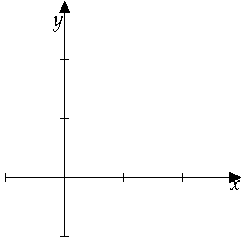
\includegraphics{plano-cartesiano.pdf}
	% \begin{tikzpicture}[line cap=round,line join=round,>=triangle 45,x=1.0cm,y=1.0cm]
	% 	\draw[->,color=black] (-1,0) -- (3,0);
	% 	\foreach \x in {-1,1,2}
	% 	\draw[shift={(\x,0)},color=black] (0pt,2pt) -- (0pt,-2pt);
	% 	\draw[color=black] (2.68,0.08) node [anchor=north west] {$x$};
	% 	\draw[->,color=black] (0,-1) -- (0,3);
	% 	\foreach \y in {-1,1,2}
	% 	\draw[shift={(0,\y)},color=black] (2pt,0pt) -- (-2pt,0pt);
	% 	\draw[color=black] (0.1,2.6) node [anchor=east] {$y$};
	% 	\clip(-1,-1) rectangle (3,3);
	% \end{tikzpicture}
\end{figure}


Seja $P$ um ponto qualquer do plano. Por $P$ podemos tra\c{c}ar uma \'unica reta $x'$ paralela \`a reta $x$ e uma \'unica reta $y'$ paralela \`a reta $y$. Estas retas interceptam $x$ e $y$ em pontos $P_x$ e $P_y$, respectivamente. Seja $\alpha$ o n\'umero real correspondente a $P_x$ e $\beta$ o n\'umero real correspondente  a $P_y$. Estes dois n\'umeros determinam o ponto $P$, isto \'e, conhecendo $\alpha$ e $\beta$ podemos tra\c{c}as as retas $x'$ e $y'$. O ponto $P$ \'e a interse\c{c}\~ao destas retas. Os n\'umeros $\alpha$ e $\beta$ s\~ao chamados \textbf{abscissa} e \textbf{ordenada} do ponto $P$, respectivamente. Eles constituem as \textbf{coordenadas} de $P$.
\begin{figure}[!h]
	\centering
	\caption{Coordenadas do ponto $P$}
	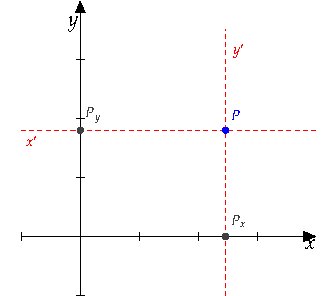
\includegraphics{coordenadas-plano-cartesiano.pdf}
	% \definecolor{uququq}{rgb}{0.25,0.25,0.25}
	% \definecolor{ffqqqq}{rgb}{1,0,0}
	% \definecolor{qqqqff}{rgb}{0,0,1}
	% \begin{tikzpicture}[line cap=round,line join=round,>=triangle 45,x=1.0cm,y=1.0cm]
	% 	\draw[->,color=black] (-1,0) -- (4,0);
	% 	\foreach \x in {-1,1,2,3}
	% 	\draw[shift={(\x,0)},color=black] (0pt,2pt) -- (0pt,-2pt);
	% 	\draw[color=black] (3.68,0.08) node [anchor=north west] {$x$};
	% 	\draw[->,color=black] (0,-1) -- (0,4);
	% 	\foreach \y in {-1,1,2,3}
	% 	\draw[shift={(0,\y)},color=black] (2pt,0pt) -- (-2pt,0pt);
	% 	\draw[color=black] (0.1,3.6) node [anchor=east] {$y$};
	% 	\clip(-1,-1) rectangle (4,4);
	% 	\draw [dash pattern=on 2pt off 2pt,color=ffqqqq] (2.46,-1) -- (2.46,3.5);
	% 	\draw [dash pattern=on 2pt off 2pt,color=ffqqqq,domain=-1:4] plot(\x,{(--1.8-0*\x)/1});
	% 	\begin{scriptsize}
	% 		\fill [color=qqqqff] (2.46,1.8) circle (1.5pt);
	% 		\draw[color=qqqqff] (2.62,2.06) node {$P$};
	% 		\draw[color=ffqqqq] (2.68,3.14) node {$y'$};
	% 		\draw[color=ffqqqq] (-0.82,1.62) node {$x'$};
	% 		\fill [color=uququq] (2.46,0) circle (1.5pt);
	% 		\draw[color=uququq] (2.68,0.26) node {$P_x$};
	% 		\fill [color=uququq] (0,1.8) circle (1.5pt);
	% 		\draw[color=uququq] (0.22,2.06) node {$P_y$};
	% 	\end{scriptsize}
	% \end{tikzpicture}
\end{figure}

Denotaremos assim o ponto $P$ por
\[
	P(\alpha,\beta).
\]

Sejam $P(x_1,y_1)$ e $Q(x_2,y_2)$ pontos do plano. A partir de $P$ e $Q$ podemos construir o tri\^angulo ret\^angulo $PQS$ como abaixo:
\begin{figure}[!h]
	\centering
	\caption{Dist\^ancia entre dois pontos}
	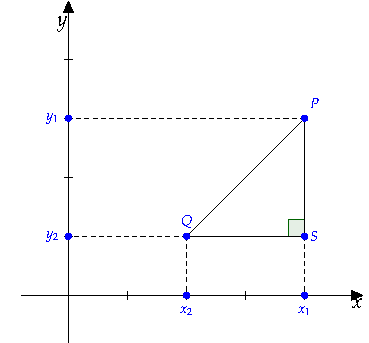
\includegraphics{distancia-pontos-plano-cartesiano.pdf}
	% \definecolor{qqwuqq}{rgb}{0,0.39,0}
	% \definecolor{xdxdff}{rgb}{0.49,0.49,1}
	% \definecolor{qqqqff}{rgb}{0,0,1}
	% \begin{tikzpicture}[line cap=round,line join=round,>=triangle 45,x=1.0cm,y=1.0cm]
	% 	\draw[->,color=black] (-0.8,0) -- (5,0);
	% 	\foreach \x in {,1,2,3,4}
	% 	\draw[shift={(\x,0)},color=black] (0pt,2pt) -- (0pt,-2pt);
	% 	\draw[color=black] (4.68,0.08) node [anchor=north west] {$x$};
	% 	\draw[->,color=black] (0,-0.8) -- (0,5);
	% 	\foreach \y in {,1,2,3,4}
	% 	\draw[shift={(0,\y)},color=black] (2pt,0pt) -- (-2pt,0pt);
	% 	\draw[color=black] (0.1,4.6) node [anchor=east] {$y$};
	% 	\clip(-0.8,-0.8) rectangle (5,5);
	% 	\draw[color=qqwuqq,fill=qqwuqq,fill opacity=0.1] (4,1.28) -- (3.72,1.28) -- (3.72,1) -- (4,1) -- cycle; 
	% 	\draw (4,1)-- (4,3);
	% 	\draw (2,1)-- (4,1);
	% 	\draw (2,1)-- (4,3);
	% 	\draw [dash pattern=on 2pt off 2pt] (4,3)-- (0,3);
	% 	\draw [dash pattern=on 2pt off 2pt] (2,1)-- (0,1);
	% 	\draw [dash pattern=on 2pt off 2pt] (2,1)-- (2,0);
	% 	\draw [dash pattern=on 2pt off 2pt] (4,1)-- (4,0);
	% 	\begin{scriptsize}
	% 		\fill [color=qqqqff] (2,1) circle (1.5pt);
	% 		\draw[color=qqqqff] (2,1.26) node {$Q$};
	% 		\fill [color=qqqqff] (4,3) circle (1.5pt);
	% 		\draw[color=qqqqff] (4.16,3.26) node {$P$};
	% 		\fill [color=qqqqff] (4,1) circle (1.5pt);
	% 		\draw[color=qqqqff] (4.16,1) node {$S$};
	% 		\fill [color=qqqqff] (0,3) circle (1.5pt);
	% 		\draw[color=qqqqff] (-0.28,3) node {$y_1$};
	% 		\fill [color=qqqqff] (0,1) circle (1.5pt);
	% 		\draw[color=qqqqff] (-0.28,1) node {$y_2$};
	% 		\fill [color=qqqqff] (2,0) circle (1.5pt);
	% 		\draw[color=qqqqff] (2,-0.26) node {$x_2$};
	% 		\fill [color=qqqqff] (4,0) circle (1.5pt);
	% 		\draw[color=qqqqff] (4,-0.26) node {$x_1$};
	% 	\end{scriptsize}
	% \end{tikzpicture}
\end{figure}

Assim sua hipotenusa \'e
\[
	\sqrt{(x_1 - x_2)^2 + (y_1 - y_2)^2}.
\]
Este n\'umero \'e chamado \textbf{dist\^ancia} de $P$ a $Q$ e \'e indicado por $d(P,Q)$, isto \'e, por defini\c{c}\~ao
\[
	d(P,Q) = \sqrt{(x_1 - x_2)^2 + (y_1 - y_2)^2}.
\]

Dizemos que dois pontos $P(x_1,y_1)$ e $Q(x_2,y_2)$ s\~ao iguais se, e somente se, $x_1 = x_2$ e $y_1 = y_2$.

% section plano_cartesiano (end)

\section{Vetores em $\real^2$} % (fold)
\label{sec:vetores_plano}

% Os vetores e as opera\c{c}\~ores com eles podem ser definidas utilizando-se do sistema de coordenadas cartesianas. Para isso, um ponto $P$ do plano \'e representado em $\real^2$ por um par de coordenadas $P(x_1, y_1)$, onde $x_1$, $y_1 \in \real$.

% Seja $\vec{u}$ um vetor no plano. Sabemos que $\vec{u}$ \'e um representante de uma certa classe de equipol\^encia dos segmentos orientados $(B,C)$. Para este segmento orientado $(B,C)$ podemos encontrar um ponto $A(x_1, y_1)$ tal que o segmento orientado $(O,A)$, onde $O(0,0)$, tem o mesmo comprimento, a mesma dire\c{c}\~ao e o mesmo sentido de $(B,C)$. Assim o vetor $\vec{u}$ pode ser representado pelo segmento orientado $(O,A)$. Portanto qualquer vetor em $\real^2$ pode ser representado como um segmento com origem no ponto $(0,0)$ e extremidade em um ponto $(x_1,y_1)$.

Sabemos que a cada par ordenado $(\alpha, \beta)$ corresponde um ponto do plano. Assim se $(\alpha, \beta) \ne (0,0)$ podemos associar uma seta com origem em $O(0,0)$ e extremidade em $(\alpha,\beta)$ como na figura abaixo:

\begin{figure}[!h]
	\centering
	\caption{Seta representando o ponto $(\alpha, \beta)$.}
	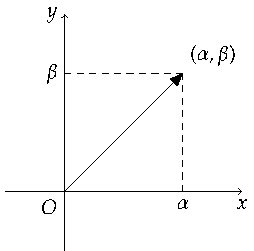
\includegraphics{vetores-plano-cartesiano.pdf}
 %  	\begin{tikzpicture}[scale=2]%vetor no plano
	%     \coordinate[label=below left:$O$] (A) at (0,0);
	%     \coordinate (W) at (1,1);
	%     %defini\c{c}\~ao das coordenadas dos eixos cartesianos
	%     \coordinate (F) at (-0.5,0);
	%     \coordinate (G) at (0,-0.5);
	%     \coordinate (X) at (1.5,0);
	%     \coordinate (Y) at (0,1.5);
	%     % Styles
	%     \tikzstyle{axes}=[]

	%     \begin{scope}[style=axes]%constr\'oi os eixos cartesianos
	% 	    \draw[->] (F) -- (X) node[below] {$x$} coordinate(x axis);
	% 	    \draw[->] (G) -- (Y) node[left] {$y$} coordinate(y axis);
	%     \end{scope}

	%     \draw[->,>=triangle 45] (A)--(W)
	%       node[above right]{$(\alpha, \beta)$};
	%     \draw[dashed,color=black] let \p1 = (W) in (\x1,0) -- (\x1,\y1)
	%       node[at start, below]{$\alpha$};
	%     \draw[dashed,color=black] let \p1 = (W) in (0,\y1) -- (\x1,\y1)
	%       node[at start, left]{$\beta$};
 %    \end{tikzpicture}
\end{figure}

Assim o par ordenado $(\alpha, \beta)$ pode ser representado graficamente por um ponto ou por uma seta. Quando representamos $(\alpha, \beta)$ por uma seta, podemos associar a este para uma \textbf{dire\c{c}\~ao}, um \textbf{sentido} e um \textbf{m\'odulo}. A dire\c{c}\~ao e o sentido do par $(\alpha, \beta)$ s\~ao respectivamente, a dire\c{c}\~ao e o sentido da seta que o representa. O \textbf{m\'odulo} do par $(\alpha, \beta)$ \'e o n\'umero
\[
	\sqrt{\alpha^2 + \beta^2}
\] 
que \'e o comprimento da seta.

Em geral, um objeto ao qual podemos associar os conceitos de dire\c{c}\~ao, sentido e m\'odulo \'e chamado um \textbf{vetor}. Denotaremos um vetor de extremidade em um ponto $(\alpha, \beta)$ por
\[
	\vec{u} = (\alpha, \beta).
\]

Esta nota\c{c}\~ao significa que $\vec{u}$ \'e a seta com in{\'\i}cio no ponto $O(0,0)$ e final no ponto $(\alpha, \beta)$.
\begin{figure}[!h]
	\centering
	\caption{Vetor $ \vec{u} = (\alpha, \beta)$.}
	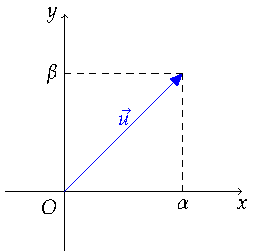
\includegraphics{vetor-coordenadas-plano-cartesiano.pdf}
  	% \begin{tikzpicture}[scale=2]%vetor no plano
	  %   \coordinate[label=below left:$O$] (A) at (0,0);
	  %   \coordinate (W) at (1,1);
	  %   %defini\c{c}\~ao das coordenadas dos eixos cartesianos
	  %   \coordinate (F) at (-0.5,0);
	  %   \coordinate (G) at (0,-0.5);
	  %   \coordinate (X) at (1.5,0);
	  %   \coordinate (Y) at (0,1.5);
	  %   % Styles
	  %   \tikzstyle{axes}=[]

	  %   \begin{scope}[style=axes]%constr\'oi os eixos cartesianos
		 %    \draw[->] (F) -- (X) node[below] {$x$} coordinate(x axis);
		 %    \draw[->] (G) -- (Y) node[left] {$y$} coordinate(y axis);
	  %   \end{scope}

	  %   \draw[->,>=triangle 45,color=blue] (A)--(W)
	  %     node[midway, above]{$\vec{u}$};
	  %   \draw[dashed,color=black] let \p1 = (W) in (\x1,0) -- (\x1,\y1)
	  %     node[at start, below]{$\alpha$};
	  %   \draw[dashed,color=black] let \p1 = (W) in (0,\y1) -- (\x1,\y1)
	  %     node[at start, left]{$\beta$};
   %  \end{tikzpicture}
\end{figure}

% Assim escrevemos $\vec{u} = \vec{OP}$. Para simplificar a nota\c{c}\~ao vamos identificar o vetor $\vec{u} = \vec{OP}$ com as coordenadas de sua extremidade e da{\'\i} escrevemos
% \[
%   \vec{u} = (x_1,y_1).
% \]
% As coordenadas $(x_1,y_1)$ s\~ao chamadas de \textbf{componentes} do vetor $\vec{u}$. Com essa representa\c{c}\~ao, o vetor nulo $\vec{0}$ \'e escrito como
% \[
%   \vec{0} = (0,0).
% \]

Por exemplo, $\vec{u} = (3,2)$ e $\vec{v} = (-1,-2)$ s\~ao representados graficamente por:
\begin{figure}[!h]
	\centering
	\caption{Vetores $\vec{u} = (3,2)$ e $\vec{v} = (-1,-2)$.}
	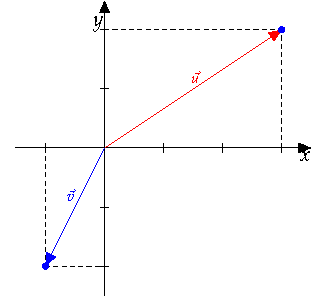
\includegraphics{exemplo-vetores-plano-cartesiano.pdf}
	% \definecolor{ffqqqq}{rgb}{1,0,0}
	% \definecolor{qqqqff}{rgb}{0,0,1}
	% \begin{tikzpicture}[line cap=round,line join=round,>=triangle 45,x=1.0cm,y=1.0cm]
	% 	\draw[->,color=black] (-1.5,0) -- (3.5,0);
	% 	\foreach \x in {-1,1,2,3}
	% 	\draw[shift={(\x,0)},color=black] (0pt,2pt) -- (0pt,-2pt);
	% 	\draw[color=black] (3.18,0.08) node [anchor=north west] {$x$};
	% 	\draw[->,color=black] (0,-2.5) -- (0,2.5);
	% 	\foreach \y in {-2,-1,1,2}
	% 	\draw[shift={(0,\y)},color=black] (2pt,0pt) -- (-2pt,0pt);
	% 	\draw[color=black] (0.1,2.1) node [anchor=east] {$y$};
	% 	\clip(-1.5,-2.5) rectangle (3.5,2.5);
	% 	\draw [->,color=ffqqqq] (0,0) -- (3,2);
	% 	\draw [->,color=qqqqff] (0,0) -- (-1,-2);
	% 	\draw [dash pattern=on 2pt off 2pt] (3,0)-- (3,2);
	% 	\draw [dash pattern=on 2pt off 2pt] (0,2)-- (3,2);
	% 	\draw [dash pattern=on 2pt off 2pt] (-1,0)-- (-1,-2);
	% 	\draw [dash pattern=on 2pt off 2pt] (-1,-2)-- (0,-2);
	% 	\begin{scriptsize}
	% 		\fill [color=qqqqff] (3,2) circle (1.5pt);
	% 		%\draw[color=qqqqff] (3.16,2.26) node {$A$};
	% 		\fill [color=qqqqff] (-1,-2) circle (1.5pt);
	% 		%\draw[color=qqqqff] (-1.16,-2.2) node {$B$};
	% 		\draw[color=ffqqqq] (1.54,1.2) node {$\vec{u}$};
	% 		\draw[color=qqqqff] (-0.58,-0.8) node {$\vec{v}$};
	% 	\end{scriptsize}
	% \end{tikzpicture}
\end{figure}

O vetor que tem in{\'\i}cio e fim no ponto $(0,0)$ \'e chamado de \textbf{vetor nulo} e ser\'a denotado por
\[
	\vec{O} = (0,0).
\]

Podemos tamb\'em representar um vetor por uma seta que n\~ao parte da origem. Por exemplo, os pontos $A(x_1,y_1)$ e $B(x_2,y_2)$ determinam o vetor
\[
	\vec{AB} = (x_2 - x_1, y_2 - y_1).
\]
\begin{figure}[!h]
	\centering
	\caption{Vetor $\vec{AB}$}
	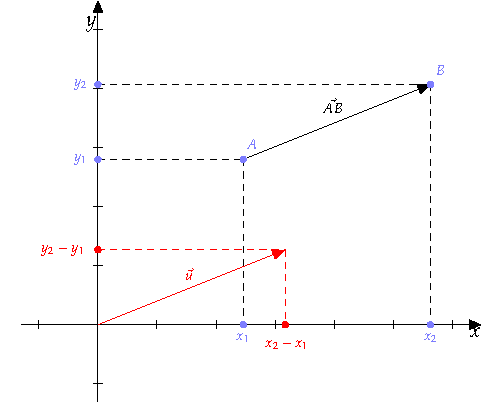
\includegraphics{vetor-AB-plano-cartesiano.pdf}
	% \definecolor{uququq}{rgb}{0.25,0.25,0.25}
	% \definecolor{ffqqqq}{rgb}{1,0,0}
	% \definecolor{xdxdff}{rgb}{0.49,0.49,1}
	% \begin{tikzpicture}[line cap=round,line join=round,>=triangle 45,x=1.0cm,y=1.0cm]
	% 	\draw[->,color=black] (-1.3,0) -- (6.5,0);
	% 	\foreach \x in {-1,1,2,3,4,5,6}
	% 	\draw[shift={(\x,0)},color=black] (0pt,2pt) -- (0pt,-2pt);
	% 	\draw[color=black] (6.18,0.08) node [anchor=north west] {$x$};
	% 	\draw[->,color=black] (0,-1.3) -- (0,5.5);
	% 	\foreach \y in {-1,1,2,3,4,5}
	% 	\draw[shift={(0,\y)},color=black] (2pt,0pt) -- (-2pt,0pt);
	% 	\draw[color=black] (0.1,5.1) node [anchor=east] {$y$};
	% 	\clip(-1.3,-1.3) rectangle (6.5,5.5);
	% 	\draw [->] (2.46,2.8) -- (5.63,4.07);
	% 	\draw [->,color=ffqqqq] (0,0) -- (3.17,1.27);
	% 	\draw [dash pattern=on 3pt off 3pt] (0,2.8)-- (2.46,2.8);
	% 	\draw [dash pattern=on 3pt off 3pt] (0,4.07)-- (5.63,4.07);
	% 	\draw [dash pattern=on 3pt off 3pt] (5.63,4.07)-- (5.63,0);
	% 	\draw [dash pattern=on 3pt off 3pt] (2.46,2.8)-- (2.46,0);
	% 	\draw [dash pattern=on 3pt off 3pt,color=ffqqqq] (0,1.27)-- (3.17,1.27);
	% 	\draw [dash pattern=on 3pt off 3pt,color=ffqqqq] (3.17,1.27)-- (3.17,0);
	% 	\begin{scriptsize}
	% 		\fill [color=xdxdff] (5.63,4.07) circle (1.5pt);
	% 		\draw[color=xdxdff] (5.8,4.32) node {$B$};
	% 		\draw[color=black] (3.98,3.72) node {$\vec{AB}$};
	% 		\draw[color=ffqqqq] (1.54,0.86) node {$\vec{u}$};
	% 		\fill [color=xdxdff] (2.46,2.8) circle (1.5pt);
	% 		\draw[color=xdxdff] (2.62,3.06) node {$A$};
	% 		\fill [color=xdxdff] (0,2.8) circle (1.5pt);
	% 		\draw[color=xdxdff] (-0.3,2.8) node {$y_1$};
	% 		\fill [color=xdxdff] (0,4.07) circle (1.5pt);
	% 		\draw[color=xdxdff] (-0.3,4.07) node {$y_2$};
	% 		\fill [color=xdxdff] (2.46,0) circle (1.5pt);
	% 		\draw[color=xdxdff] (2.46,-0.22) node {$x_1$};
	% 		\fill [color=xdxdff] (5.63,0) circle (1.5pt);
	% 		\draw[color=xdxdff] (5.63,-0.22) node {$x_2$};
	% 		\fill [color=ffqqqq] (3.17,0) circle (1.5pt);
	% 		\draw[color=ffqqqq] (3.2,-0.32) node {$x_2-x_1$};
	% 		\fill [color=ffqqqq] (0,1.27) circle (1.5pt);
	% 		\draw[color=ffqqqq] (-0.6,1.27) node {$y_2-y_1$};
	% 	\end{scriptsize}
	% \end{tikzpicture}
\end{figure}

Assim a seta que representa o vetor $\vec{AB}$ e a seta que representa o vetor $\vec{u}$, que tem in{\'\i}cio na origem e extremidade no ponto $(x_2 - x_1, y_2 - y_1)$, t\^em o mesmo m\'odulo, dire\c{c}\~ao e sentido que $\vec{AB}$. Assim vamos representar o vetor $\vec{AB}$ pela forma que for mais conveniente.

\begin{definicao}
  Seja $\vec{u} = (x_1, y_1)$ um vetor. A \textbf{norma} de $\vec{u}$, denotada por $\norm{\vec{u}}$, \'e dada por
  \[
    \norm{\vec{u}} = \sqrt{x_1^2 + y_1^2}.
  \]
\end{definicao}

Um vetor $\vec{u}$ tal que
\[
	\norm{\vec{u}} = 1
\]
\'e chamado de \textbf{vetor unit\'ario}.
\begin{figure}[!h]
	\centering
	\caption{Vetores unit\'arios: $\norm{\vec{u}} = 1$}
	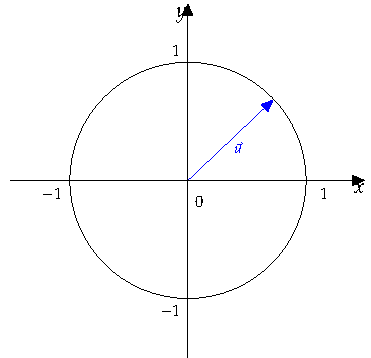
\includegraphics{vetores-unitarios-plano-cartesiano.pdf}
	% \definecolor{qqqqff}{rgb}{0,0,1}
	% \begin{tikzpicture}[line cap=round,line join=round,>=triangle 45,x=1.0cm,y=1.0cm]
	% 	\draw[->,color=black] (-3,0) -- (3,0);
	% 	\draw (-2.3,0) node[below] {\footnotesize $-1$};
	% 	\draw (2.3,0) node[below] {\footnotesize $1$};
	% 	\draw (0,2.2) node[left] {\footnotesize $1$};
	% 	\draw (0,-2.2) node[left] {\footnotesize $-1$};
	% 	\draw[color=black] (2.68,0.08) node [anchor=north west] {$x$};
	% 	\draw[->,color=black] (0,-3) -- (0,3);
	% 	\draw[color=black] (0.1,2.8) node [anchor=east] {$y$};
	% 	\draw[color=black] (0pt,-10pt) node[right] {\footnotesize $0$};
	% 	\clip(-3,-3) rectangle (3,3);
	% 	\draw(0,0) circle (2cm);
	% 	\draw [->,color=qqqqff] (0,0) -- (1.45,1.37);
	% 	\begin{scriptsize}
	% 		\draw[color=qqqqff] (0.84,0.56) node {$\vec{u}$};
	% 	\end{scriptsize}
	% \end{tikzpicture}
\end{figure}

\begin{definicao}
	Dois vetores $\vec{u}$ e $\vec{v}$ s\~ao \textbf{paralelos} (ou \textbf{colineares}) se a restas que cont\'em estes vetores s\~ao paralelas(podendo ser coincidentes).Caso $\vec{u}$ e $\vec{v}$ sejam paralelos, escreveremos $\vec{u}\varparallel\vec{v}$. Neste caso, $\vec{u}$ e $\vec{v}$ t\^em a mesma dire\c{c}\~ao, mas podem ter sentidos contr\'arios.
\end{definicao}
\begin{figure}[!h]
	\centering
	\caption{Vetores paralelos}
	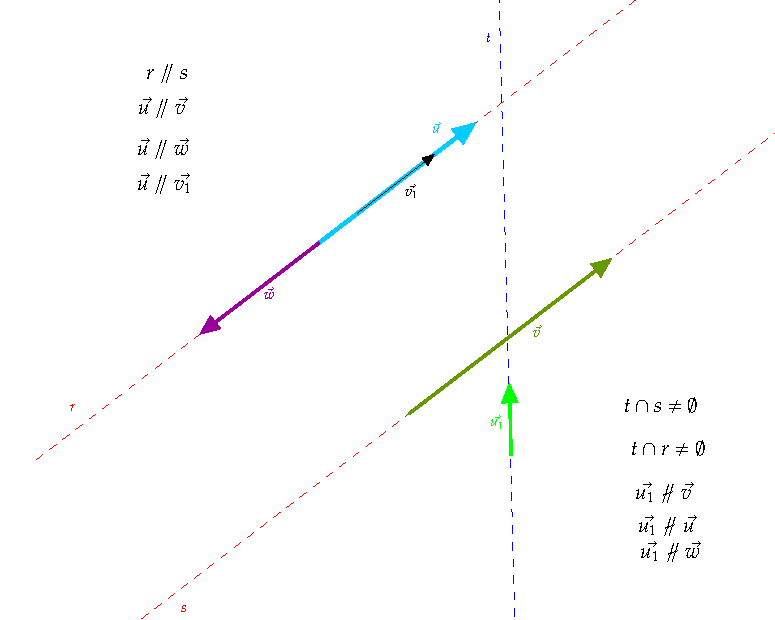
\includegraphics{vetores-paralelos-plano-cartesiano.pdf}
	% \definecolor{qqffqq}{rgb}{0,1,0}
	% \definecolor{qqqqff}{rgb}{0,0,1}
	% \definecolor{zzqqzz}{rgb}{0.6,0,0.6}
	% \definecolor{wwzzqq}{rgb}{0.4,0.6,0}
	% \definecolor{qqccff}{rgb}{0,0.8,1}
	% \definecolor{ffqqqq}{rgb}{1,0,0}
	% \begin{tikzpicture}[line cap=round,line join=round,>=triangle 45,x=1.0cm,y=1.0cm]
	% 	\clip(-3.5,-4.5) rectangle (9,6);
	% 	\draw [dash pattern=on 4pt off 4pt,color=ffqqqq,domain=-3.5:9] plot(\x,{(--2.39--2.04*\x)/2.66});
	% 	\draw [dash pattern=on 4pt off 4pt,color=ffqqqq,domain=-3.5:9] plot(\x,{(-8.41--2.04*\x)/2.66});
	% 	\draw [->,line width=1.6pt,color=qqccff] (1.28,1.88) -- (3.94,3.92);
	% 	\draw [->,line width=1.2pt,color=wwzzqq] (2.82,-1) -- (6.24,1.62);
	% 	\draw [->,line width=1.2pt,color=zzqqzz] (1.28,1.88) -- (-0.73,0.34);
	% 	\draw [dash pattern=on 4pt off 4pt,color=qqqqff,domain=-3.5:9] plot(\x,{(--8.89-1.98*\x)/0.05});
	% 	\draw [->,line width=1.2pt,color=qqffqq] (4.54,-1.7) -- (4.51,-0.49);
	% 	\draw [->] (1.94,2.39) -- (3.25,3.39);
	% 	\draw (-1.76,5.04) node[anchor=north west] {$ r\varparallel s $};
	% 	\draw (-1.9,4.48) node[anchor=north west] {$\vec{u}\varparallel \vec{v}$};
	% 	\draw (-1.92,3.78) node[anchor=north west] {$\vec{u}\varparallel \vec{w}$};
	% 	\draw (-1.92,3.2) node[anchor=north west] {$\vec{u}\varparallel \vec{v_1}$};
	% 	\draw (6.32,-0.6) node[anchor=north west] {$ t \cap s \ne \emptyset $};
	% 	\draw (6.44,-1.32) node[anchor=north west] {$ t \cap r \ne \emptyset $};
	% 	\draw (6.52,-2.04) node[anchor=north west] {$\vec{u_1}\nvarparallel \vec{v}$};
	% 	\draw (6.56,-2.6) node[anchor=north west] {$\vec{u_1}\nvarparallel \vec{u}$};
	% 	\draw (6.6,-3.04) node[anchor=north west] {$\vec{u_1}\nvarparallel \vec{w}$};
	% 	\begin{scriptsize}
	% 		\draw[color=ffqqqq] (-2.88,-0.9) node {$r$};
	% 		\draw[color=ffqqqq] (-1,-4.3) node {$s$};
	% 		\draw[color=qqccff] (3.26,3.84) node {$\vec{u}$};
	% 		\draw[color=wwzzqq] (4.98,0.4) node {$\vec{v}$};
	% 		\draw[color=zzqqzz] (0.44,1.04) node {$\vec{w}$};
	% 		\draw[color=qqqqff] (4.16,5.36) node {$t$};
	% 		\draw[color=qqffqq] (4.3,-1.14) node {$\vec{u_1}$};
	% 		\draw[color=black] (2.86,2.76) node {$\vec{v_1}$};
	% 	\end{scriptsize}
	% \end{tikzpicture}
\end{figure}

\subsection{Opera\c{c}\~oes com Vetores} % (fold)
\label{sub:operacoes_com_vetores}

\begin{definicao}
  Sejam $\vec{u} = (x_1, y_1)$ e $\vec{v} = (x_2, y_2)$ vetores. Ent\~ao:
  \[
  	\vec{u} + \vec{v} = (x_1 + x_2, y_1 + y_2).
  \]
\end{definicao}

\begin{figure}[!h]
  \centering
  \caption{Soma de vetores}
  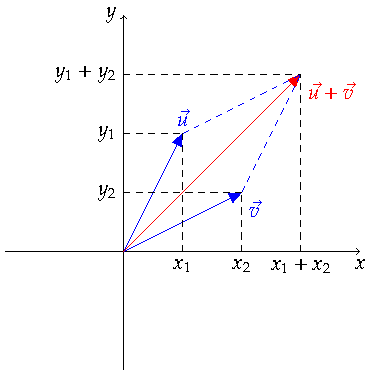
\includegraphics{soma-vetores-plano-cartesiano.pdf}
  % \begin{tikzpicture}[scale=2]%soma de vetores no plano
  %   \coordinate (A) at (0,0);
  %   \coordinate (V) at (0.5,1);
  %   \coordinate (W) at (1,0.5);
  %   \coordinate (B) at (0,1);
  %   \coordinate (VW) at ($(V)+(W)$);
  %   %defini\c{c}\~ao das coordenadas dos eixos cartesianos
  %   \coordinate (F) at (-1,0);
  %   \coordinate (G) at (0,-1);
  %   \coordinate (X) at (2,0);
  %   \coordinate (Y) at (0,2);
  %   % Styles
  %   \tikzstyle{axes}=[]

  %   \begin{scope}[style=axes]%constr\'oi os eixos cartesianos
  %   \draw[->] (F) -- (X) node[below] {$x$} coordinate(x axis);
  %   \draw[->] (G) -- (Y) node[left] {$y$} coordinate(y axis);
  %   \end{scope}

  %   \draw[->,>=triangle 45,color=blue] (A)--(V)
  %     node[above]{$\vec{u}$};
  %   \draw[->,>=triangle 45,color=blue] (A)--(W)
  %     node[below right]{$\vec{v}$};
  %   \draw[->,>=triangle 45,color=red] (A)--(VW)
  %     node[below right]{$\vec{u}+\vec{v}$};
  %   \draw[dashed,>=triangle 45,color=blue] (V)--(VW);
  %   \draw[dashed,>=triangle 45,color=blue] (W)--(VW);
  %   \draw[dashed,color=black] let \p1 = (V) in (\x1,0) -- (\x1,\y1)
  %     node[at start, below]{$x_1$};
  %   \draw[dashed,color=black] let \p1 = (V) in (0,\y1) -- (\x1,\y1)
  %     node[at start, left]{$y_1$};
  %   \draw[dashed,color=black] let \p1 = (W) in (\x1,0) -- (\x1,\y1)
  %     node[at start, below]{$x_2$};
  %   \draw[dashed,color=black] let \p1 = (W) in (0,\y1) -- (\x1,\y1)
  %     node[at start, left]{$y_2$};
  %   \draw[dashed,color=black] let \p1 = (VW) in (\x1,0) -- (\x1,\y1)
  %     node[at start, below]{$x_1 + x_2$};
  %   \draw[dashed,color=black] let \p1 = (VW) in (0,\y1) -- (\x1,\y1)
  %     node[at start, left]{$y_1 + y_2$};
  % \end{tikzpicture}
\end{figure}

\begin{propriedades}\label{propriedades_soma_vetores}
  Sejam $\vec{u}$, $\vec{v}$ e $\vec{w}$ vetores quaisquer. As seguintes propriedades s\~ao verdadeiras:
  \begin{enumerate}[label=({\roman*})]
    \item $(\vec{u} + \vec{v}) + \vec{w} = \vec{u} + (\vec{v} + \vec{w})$ [Associatividade]
    \item $\vec{u} + \vec{v} = \vec{v} + \vec{u}$ [Comutatividade]
    \item Existe um \'unico vetor que somado a $\vec{u}$ resulta no pr\'oprio vetor $\vec{u}$:
    \[
      \vec{u} + \vec{0} = \vec{0} + \vec{u} = \vec{u}.
    \]
    Tal vetor \'e o vetor nulo. [Elementro Neutro]
    \item\label{vetor_oposto} Para cada $\vec{u}$, existe um \'unico vetor $\vec{v}$ tal que
    \[
      \vec{u} + \vec{v} = \vec{0} = \vec{v} + \vec{u}.
    \]
    O vetor $\vec{v}$ \'e o vetor oposto de $\vec{u}$. [Elemento Oposto]
  \end{enumerate}
\end{propriedades}
\begin{prova}
	Sejam $\vec{u} = (x_1,y_1)$, $\vec{v} = (x_2,y_2)$ e $\vec{w} = (x_3,y_3)$. Temos
	\begin{enumerate}[label=({\roman*})]
		\item $(\vec{u} + \vec{v}) + \vec{w} = (x_1+x_2,y_1+y_2) + \vec{w} = ((x_1+x_2)+x_3,(y_1+y_2)+y_3) = (x_1+(x_2+x_3),y_1+(y_2+y_3)) = \vec{u} + (x_2+x_3,y_2+y_3) = \vec{u} + (\vec{v} + \vec{w})$.
		\item $\vec{u} + \vec{v} = (x_1+x_2,y_1+y_2) = (x_2+x_1,y_2+y_1) = \vec{v} + \vec{u}$.
		\item Usando o item (A2) basta verificar que $\vec{u} + \vec{0} = \vec{u}$. De fato
		\[
      		\vec{u} + \vec{0} = (x_1,y_1) + (0,0) = (x_1,y_1) = \vec{u}.
    	\]
    	\item Novamente, pelo item (A2) basta verificar que $\vec{u} + \vec{v} = \vec{0}$. De fato, dado $\vec{u} = (x_1,y_1)$, tomando $\vec{v} = (-x_1,-y_1)$ temos
    	\[
    		\vec{u} + \vec{v} = (x_1,y_1) + (-x_1,-y_1) = (0,0) = \vec{0}.
    	\]
	\end{enumerate}
	Portanto as propriedades s\~ao verdadeiras.
\end{prova}

\begin{definicao}
	O vetor $\vec{v}$ do item \ref{vetor_oposto} da Defini\c{c}\~ao \ref{propriedades_soma_vetores} \'e chamado de \textbf{vetor oposto}.
\end{definicao}


\begin{definicao}
  Sejam $\alpha \in \real$, $\vec{u} = (x_1, y_1)$ e $\vec{v} = (x_2, y_2)$ vetores. Ent\~ao:
  \[
  	\alpha \vec{u} = (\alpha x_1, \alpha y_1).
  \]
\end{definicao}

\begin{figure}[!h]
  \centering
  \caption{Multiplica\c{c}\~ao por escalar}
  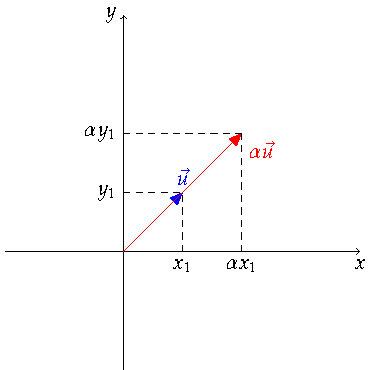
\includegraphics{multiplicacao-escalar-vetores-plano-cartesiano.pdf}
  % \begin{tikzpicture}[scale=2]%multiplica\c{c}\~ao por escalar no plano
  %   \coordinate (A) at (0,0);
  %   \coordinate (V) at (0.5,0.5);
  %   \coordinate (W) at ($2*(V)$);
  %   %defini\c{c}\~ao das coordenadas dos eixos cartesianos
  %   \coordinate (F) at (-1,0);
  %   \coordinate (G) at (0,-1);
  %   \coordinate (X) at (2,0);
  %   \coordinate (Y) at (0,2);
  %   % Styles
  %   \tikzstyle{axes}=[]

  %   \begin{scope}[style=axes]%constr\'oi os eixos cartesianos
	 %    \draw[->] (F) -- (X) node[below] {$x$} coordinate(x axis);
	 %    \draw[->] (G) -- (Y) node[left] {$y$} coordinate(y axis);
  %   \end{scope}

  %   \draw[->,>=triangle 45,color=blue] (A)--(V)
  %     node[above]{$\vec{u}$};
  %   \draw[->,>=triangle 45,color=red] (A)--(W)
  %     node[below right]{$\alpha \vec{u}$};
  %   \draw[dashed,color=black] let \p1 = (V) in (\x1,0) -- (\x1,\y1)
  %     node[at start, below]{$x_1$};
  %   \draw[dashed,color=black] let \p1 = (V) in (0,\y1) -- (\x1,\y1)
  %     node[at start, left]{$y_1$};
  %   \draw[dashed,color=black] let \p1 = (W) in (\x1,0) -- (\x1,\y1)
  %     node[at start, below]{$\alpha x_1$};
  %   \draw[dashed,color=black] let \p1 = (W) in (0,\y1) -- (\x1,\y1)
  %     node[at start, left]{$\alpha y_1$};
  % \end{tikzpicture}
\end{figure}

\begin{observacao}
	\begin{enumerate}
		\item Sejam $\vec{u}$ um vetor n\~ao-nulo e $\lambda \ne 0$ um escalar. Ent\~ao $\vec{u} \varparallel\lambda\vec{u}$. Al\'em disso, se $\lambda > 0$, ent\~ao $\vec{u}$ e $\lambda\vec{u}$ s\~ao de mesmo sentido, e se $\lambda < 0$ ent\~ao $\vec{u}$ e $\lambda\vec{u}$ s\~ao de sentidos contr\'arios.
		\item Quando $\lambda = -1$, o vetor $-\vec{u} = (-x_1,-y_1)$  \'e exatamente o vetor oposto de $\vec{u}$. Note que $-\vec{u}$ tem a mesma dire\c{c}\~ao que $\vec{u}$, mas sentido contr\'ario.
	\end{enumerate}
	
\end{observacao}

\begin{propriedades}
  Quaisquer que sejam os n\'umeros reais $\alpha$ e $\beta$ e quaisquer que sejam os vetores $\vec{u}$ e $\vec{v}$ valem as igualdades:
  \begin{enumerate}[label=({\roman*})]
    \item $\alpha(\vec{u} + \vec{v}) = \alpha\vec{u} + \alpha\vec{v}$;
    \item $(\alpha + \beta)\vec{u} = \alpha\vec{u} + \beta\vec{u}$;
    \item $1\vec{u} = \vec{u}$;
    \item $\alpha(\beta\vec{u}) = (\alpha\beta)\vec{u} = \beta(\alpha\vec{u})$.
  \end{enumerate}
\end{propriedades}
\begin{prova}
	Sejam $\vec{u} = (x_1,y_1)$ e $\vec{v} = (x_2,y_2)$. Temos:
	\begin{enumerate}[label=({\roman*})]
		\item $\alpha(\vec{u} + \vec{v}) = \alpha(x_1+x_2,y_1+y_2) = (\alpha(x_1+x_2),\alpha(y_1+y_2)) = (\alpha x_1,\alpha y_1) + (\alpha x_2,\alpha y_2) =  \alpha\vec{u} + \alpha\vec{v}$.
		\item $(\alpha + \beta)\vec{u} = ((\alpha+\beta)x_1,(\alpha+\beta)y_1) = (\alpha x_1 + \beta x_1, \alpha y_1 + \beta y_1) = (\alpha x_1,\alpha y_1) + (\beta x_1,\beta y_1) = \alpha\vec{u} + \beta\vec{u}$.
		\item $1\vec{u} = 1(x_1,y_1) = (x_1,y_1) = \vec{u}$.
		\item Primeiro temos:
		\[
			\alpha(\beta\vec{u}) = \alpha(\beta x_1,\beta y_1) = (\alpha(\beta x_1),\alpha(\beta y_1)) = ((\alpha\beta)x_1,(\alpha\beta)y_1) = (\alpha\beta)\vec{u}.
		\]
		Agora,
		\[
			(\alpha\beta)\vec{u} = 	((\alpha\beta)x_1,(\alpha\beta)y_1) = ((\beta\alpha)x_1,(\beta\alpha)y_1) = (\beta(\alpha x_1),\beta(\alpha y_1)) = \beta(\alpha\vec{u}).
		\]
		Logo $\alpha(\beta\vec{u}) = (\alpha\beta)\vec{u} = \beta(\alpha\vec{u})$.
	\end{enumerate}
	Portanto as propriedades s\~ao v\'alidas.
\end{prova}

% \begin{proposicao}
%   Quaisquer que sejam o escalar $\alpha$ e o vetor $\vec{u}$, valem as seguintes igualdades:
%   \begin{enumerate}[label=({\roman*})]
%     \item $(-\alpha)\vec{u} = -(\alpha\vec{u})$;
%     \item $\alpha(-\vec{u}) = -(\alpha\vec{u})$;
%     \item $(-\alpha)(-\vec{u}) = \alpha\vec{u}$.
%   \end{enumerate}
% \end{proposicao}

Em alguns casos pode ser mais conveniente representar um vetor $\vec{u} = (x_1, y_1)$ de forma matricial. Para isso escrevemos as componentes de $\vec{u}$ como uma matriz de 1 coluna e duas linhas
\[
  \vec{u} = \begin{bmatrix}
    x_1\\y_1
  \end{bmatrix}.
\]

%Vimos que a norma de um vetor \'e definida como o comprimento de um segmento orientado que o represente. Com a representa\c{c}\~ao de vetores por coordenadas podemos reescrever o conceito de norma da seguinte maneira:

\begin{exemplos}
  Seja $\vec{u} = (-2,3)$ um vetor. Ent\~ao
  \begin{align*}
    \norm{\vec{u}} &= \sqrt{(-2)^2 + 3^2} = \sqrt{13}\\
    \vec{v} &= \dfrac{\vec{u}}{\norm{u}} = \dfrac{1}{\sqrt{13}}(-2,3) = \left(\dfrac{-2}{\sqrt{13}}, \dfrac{3}{\sqrt{13}}\right).
  \end{align*}
\end{exemplos}


% subsection operacoes_com_vetores (end)


% section vetores_plano (end)

\begin{proposicao}
  Sejam $\vec{u} = (x_1, y_1)$ um vetor em $\real^2$ e $\alpha \in \real$. Ent\~ao:
  \begin{enumerate}
    \item Se $\vec{u} \ne \vec{0}$, ent\~ao $\norm{\vec{u}} \ne 0$.
    \item $\norm{\vec{u}} = 0$ se, e somente se, $\vec{u} = \vec{0}$.
    \item $\norm{\alpha\vec{u}} = |\alpha|\norm{\vec{u}}$.
  \end{enumerate}
\end{proposicao}
\begin{prova}
  \begin{enumerate}
    \item  Se $\vec{u} \ne (0,0) = \vec{0}$, ent\~ao $x_1 \ne 0$ ou $y_1 \ne 0$. Da{\'\i}
    \[
      \norm{\vec{u}} = \sqrt{x_1^2 + y_1^2} > 0.
    \]
    \item $\norm{\vec{u}} = 0$ se, e somente se, $x_1^2 + y_1^2 = 0$, isto \'e, $x_1 = y_1 = 0$. Portanto $\vec{u} = \vec{0}$.
    \item $\norm{\alpha\vec{u}} = \norm{\alpha(x_1, y_1)} = \sqrt{(\alpha x_1)^2 + (\alpha y_1)^2} = \sqrt{\alpha^2(x_1^2 + y_1^2)} = |\alpha|\norm{\vec{u}}$.
  \end{enumerate}
\end{prova}

\begin{observacao}
	Dado um vetor n\~ao nulo $\vec{u}$ o vetor
	\[
  		\vec{v} = \dfrac{\vec{u}}{\norm{\vec{u}}}
	\]
	\'e um vetor unit\'ario na dire\c{c}\~ao de $\vec{u}$ pois
	\[
  		\norm{\vec{v}} = \norm{\dfrac{\vec{u}}{\norm{\vec{u}}}} = \dfrac{1}{\norm{\vec{u}}}\norm{\vec{u}} = 1.
	\]

\end{observacao}
\begin{definicao}
	Sejam $\vec{u}$ e $\vec{v}$ vetores n\~ao-nulos. Ent\~ao $\vec{u} = \vec{v}$ se, e somente se, $\vec{u}$ e $\vec{v}$ t\^em normas iguais, s\~ao de mesma dire\c{c}\~ao e de mesmo sentido.
\end{definicao}

\begin{proposicao}\label{vetores_paralelos}
  Dois vetores n\~ao nulos $\vec{u}$ e $\vec{v}$ s\~ao paralelos se, e somente se, existe um escalar $\lambda$ tal que $\vec{u} = \lambda\vec{v}$ (consequentemente, $\lambda \ne 0$ e assim $\vec{v} = \vec{u}/\lambda$).
\end{proposicao}
\begin{prova}
	Se $\vec{u} = \lambda\vec{v}$, ent\~ao $\vec{u}\varparallel\vec{v}$.
	Agora, suponha que $\vec{u}$ e $\vec{v}$ s\~ao paralelos e de mesmo sentido, o caso em que t\^em sentidos contr\'arios fica como exerc{\'\i}cio.

	Seja 
	\[
		\lambda = \dfrac{\norm{\vec{u}}}{\norm{\vec{v}}}.
	\]
	Vamos mostrar que $\vec{u} = \lambda\vec{v}$. Inicialmente, sabemos que $\vec{v}$ e $\lambda\vec{v}$ s\~ao paralelos e t\^em o mesmo sentido pois $\lambda > 0$. Agora
	\[
		\norm{\lambda\vec{v}} = |\lambda|\norm{\vec{v}} = \dfrac{\norm{\vec{u}}}{\norm{\vec{v}}}\norm{\vec{v}} = \norm{\vec{u}}.
	\]
	Portanto $\vec{u}$ e $\lambda\vec{v}$ tem a mesma dire\c{c}\~ao, o mesmo sentido e normas iguais, logo $\vec{u} = \lambda\vec{v}$, como quer{\'\i}amos.
\end{prova}

\subsection{\^Angulo entre vetores e produto interno} % (fold)
\label{sub:angulo_entre_vetores_e_produto_interno}
\begin{definicao}
  Sejam $\vec{u}$ e $\vec{v}$ vetores n\~ao nulos. O \textbf{\^angulo} entre $\vec{u}$ e $\vec{v}$ \'e definido pelo \^angulo $\theta$ determinado por $\vec{u}$ e $\vec{v}$ e que satisfaz $0 \le \theta \le \pi$, quando os vetores $\vec{u}$ e $\vec{v}$ s\~ao representados com a mesma origem.\index{Vetores!\^Angulo}
\end{definicao}

\begin{figure}[!h]
  \centering
  \caption{\^Angulo entre vetores}
  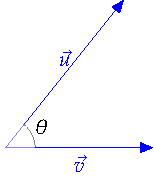
\includegraphics{angulo-vetores-plano-cartesiano.pdf}
  % \begin{tikzpicture}
  %   \coordinate (A) at (0,0);
  %   \coordinate (X) at (2.5,0);
  %   \coordinate (Y) at (2,2.5);

  %   \draw[->,>=triangle 45,color=blue] (A) -- (X)
  %     node[midway,below]{$\vec{v}$};
  %   \draw[->,>=triangle 45,color=blue] (A) -- (Y)
  %     node[midway,above]{$\vec{u}$};
  % % \draw[dashed,->,>=triangle 45] (X) -- (Y)
  %   % node[midway,above right]{$\vec{u} - \vec{v}$};

  %   % Mark the angle XAY
  %   \begin{scope}
  %     \path[clip] (A) -- (X) -- (Y);
  %     \fill[white, opacity=0.5, draw=black] (A) circle (5mm);
  %     \node at ($(A)+(30:7mm)$) {$\theta$};
  %   \end{scope}
  % \end{tikzpicture}
\end{figure}


\begin{definicao}
  Quando o \^angulo $\theta$ entre dois vetores $\vec{u}$ e $\vec{v}$ \'e reto, isto \'e, $\theta = \pi/2$, ou um deles \'e o vetor nulo, dizemos que os vetores $\vec{u}$ e $\vec{v}$ s\~ao \textbf{ortogonais} ou \textbf{perpendiculares} entre si. Denotamos tal fato, escrevendo $\vec{u} \perp \vec{v}$.\index{Vetores!Ortogonais}
\end{definicao}

Sejam $\vec{u}$ e $\vec{v}$ vetores n\~ao nulos e $\theta$ o \^angulo entre eles.
\begin{figure}[!h]
  \centering
  \caption{Determina\c{c}\~ao de $\theta$}
  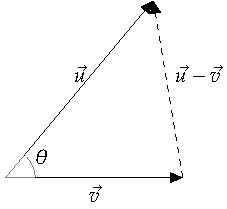
\includegraphics{determinacao-angulo-vetores-plano-cartesiano.pdf}
  % \begin{tikzpicture}
  %   \coordinate (A) at (0,0);
  %   \coordinate (X) at (3,0);
  %   \coordinate (Y) at (2.5,3);

  %   \draw[->,>=triangle 45] (A) -- (X)
  %   node[midway,below]{$\vec{v}$};
  %   \draw[->,>=triangle 45] (A) -- (Y)
  %   node[midway,above]{$\vec{u}$};
  %   \draw[dashed,->,>=triangle 45] (X) -- (Y)
  %   node[midway,above right]{$\vec{u} - \vec{v}$};

  %   % Mark the angle XAY
  %   \begin{scope}
  %     \path[clip] (A) -- (X) -- (Y);
  %     \fill[white, opacity=0.5, draw=black] (A) circle (5mm);
  %     \node at ($(A)+(30:7mm)$) {$\theta$};
  %   \end{scope}
  % \end{tikzpicture}
\end{figure}

Aplicando a Lei dos cosssenos no tri\^angulo abaixo
\begin{figure}[!h]
  \centering
  \caption{Lei dos cossenos}
  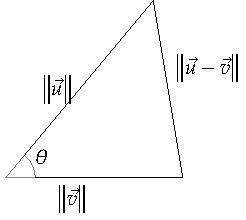
\includegraphics{lei-cossenos-vetores-plano-cartesiano.pdf}
  % \begin{tikzpicture}
  %   \coordinate (A) at (0,0);
  %   \coordinate (X) at (3,0);
  %   \coordinate (Y) at (2.5,3);

  %   \draw (A) -- (X)
  %   node[midway,below left]{$\norm{\vec{v}}$};
  %   \draw(A) -- (Y)
  %   node[midway,left]{$\norm{\vec{u}}$};
  %   \draw(X) -- (Y)
  %   node[midway,above right]{$\norm{\vec{u} - \vec{v}}$};

  %   % Mark the angle XAY
  %   \begin{scope}
  %     \path[clip] (A) -- (X) -- (Y);
  %     \fill[white, opacity=0.5, draw=black] (A) circle (5mm);
  %     \node at ($(A)+(30:7mm)$) {$\theta$};
  %   \end{scope}
  % \end{tikzpicture}
\end{figure}
temos
\begin{align}\label{equacaonorma}
  \norm{\vec{u} - \vec{v}}^2 = \norm{\vec{u}}^2 + \norm{\vec{v}}^2 - 2\norm{\vec{u}}\norm{\vec{v}}\cos\theta.
\end{align}

% Assim conhecendo as coordenadas dos vetores $\vec{u}$ e $\vec{v}$ podemos determinar facilmente o \^angulo entre eles. Al\'em disso, note que se $\vec{u}$ e $\vec{v}$ s\~ao vetores ortogonais, ent\~ao $\theta = \pi/2$ e ent\~ao a equa\c{c}\~ao \eqref{equacaonorma} torna-se
% \begin{align}\label{norma-vetores-ortogonais}
%   \norm{\vec{u} - \vec{v}} = \sqrt{\norm{\vec{u}}^2 + \norm{\vec{v}}^2}.
% \end{align}

% \begin{observacao}
%   A equa\c{c}\~ao \eqref{norma-vetores-ortogonais} s\'o \'e v\'alida para vetores ortogonais entre si.
% \end{observacao}

\begin{definicao}\label{produtointerno}
  O \textbf{produto escalar} ou \textbf{produto interno} dos vetores $\vec{u}$ e $\vec{v}$, indicado por $\vec{u}\cdot\vec{v}$, \'e o n\'umero real tal que:\index{Vetores!Produto Escalar}
  \begin{enumerate}
    \item Se $\vec{u}$ ou $\vec{v}$ \'e nulo, ent\~ao $\vec{u}\cdot\vec{v} = 0$.
    \item Se $\vec{u}$ e $\vec{v}$ n\~ao s\~ao nulos e $\theta$ \'e o \^angulo entre $\vec{u}$ e $\vec{v}$, ent\~ao
    \begin{align}\label{produto-interno}
      \vec{u}\cdot\vec{v} = \norm{\vec{u}}\norm{\vec{v}}\cos\theta.
    \end{align}
  \end{enumerate}
\end{definicao}

\begin{proposicao}
  Sejam $\vec{u}$ e $\vec{v}$ vetores e $\theta$ o \^angulo entre $\vec{u}$ e $\vec{v}$.
  \begin{enumerate}
    \item Se $\vec{u}$ e $\vec{v}$ n\~ao s\~ao nulos, ent\~ao
    \[
      \cos\theta = \dfrac{\vec{u}\cdot\vec{v}}{\norm{\vec{u}}\norm{\vec{v}}}.
    \]
    \item Qualquer que seja o vetor $\vec{u}$,
    \[
      \norm{\vec{u}} = \sqrt{\vec{u}\cdot\vec{u}}.
    \]
    \item Quaisquer que sejam os vetores $\vec{u}$ e $\vec{v}$, $\vec{u}\perp\vec{v}$ se, e somente se, $\vec{u}\cdot\vec{v} = 0$.
    \end{enumerate}
\end{proposicao}
\begin{prova}
  \begin{enumerate}
    \item Basta isolar $\cos\theta$ na Defini\c{c}\~ao \ref{produto-interno}.
    \item Se $\vec{u} = \vec{0}$, ent\~ao a igualdade \'e verdadeira. Se $\vec{u} \ne \vec{0}$, ent\~ao o \^angulo entre o vetor $\vec{u}$ e ele mesmo \'e $\theta = 0$, logo
    \[
      1 = \cos\theta = \dfrac{\vec{u}\cdot\vec{u}}{\norm{\vec{u}}\norm{\vec{u}}}.
    \]
    Logo
    \[
      \norm{\vec{u}} = \sqrt{\vec{u}\cdot\vec{u}}.
    \]
    \item Se $\vec{u}$ ou $\vec{v}$ \'e o vetor nulo, ent\~ao $\vec{u}\perp\vec{v}$ e $\vec{u}\cdot\vec{v} = 0$. Suponha $\vec{u} \ne \vec{0}$ e $\vec{v} \ne \vec{0}$. Assim, se $\vec{u} \perp\vec{v}$, ent\~ao $\theta = \pi/2$ e da{\'\i} $\vec{u}\cdot\vec{v} = 0$. Agora, se $\vec{u}\cdot\vec{v} = 0$, ent\~ao
    \[
      0 = \vec{u}\cdot\vec{v} = \norm{\vec{u}}\norm{\vec{v}}\cos\theta.
    \]
    Logo devemos ter $\cos\theta = 0$, isto \'e, $\theta = \pi/2$. Portanto $\vec{u}\perp\vec{v}$, como quer{\'\i}amos.
  \end{enumerate}
\end{prova}

Agora, como podemos encontrar o produto interno sem necessitar de determinar o \^angulo $\theta$ entre dois vetores $\vec{u}$ e $\vec{v}$? Substituindo o produto interno na equa\c{c}\~ao \eqref{equacaonorma} temos
\[
  \norm{\vec{u} - \vec{v}}^2 = \norm{\vec{u}}^2 + \norm{\vec{v}}^2 - 2\vec{u}\cdot\vec{v}
\]
isto \'e,
\begin{align}\label{equacao-auxilar-norma}
  \vec{u}\cdot\vec{v} = \dfrac{1}{2}(\norm{\vec{u}}^2 + \norm{\vec{v}}^2 - \norm{\vec{u} - \vec{v}}^2).
\end{align}
Se $\vec{u} = (x_1, y_1)$ e $\vec{v} = (x_2, y_2)$, ent\~ao podemos reescrever \eqref{equacao-auxilar-norma} como
\begin{align*}
  \vec{u}\cdot\vec{v} &= \dfrac{1}{2}(x_1^2 + y_1^2 + x_2^2 + y_2^2 - \norm{(x_1 - x_2, y_1 - y_2)}^2)\\
  &= \dfrac{1}{2}[x_1^2 + y_1^2 + x_2^2 + y_2^2 - (x_1 - x_2)^2 - (y_1 - y_2)^2]\\
  &= x_1x_2 + y_1y_2.
\end{align*}

Abacamos de demonstrar o seguinte teorema:
\begin{teorema}
  O produto interno de dois vetores $\vec{u} = (x_1, y_1)$ e $\vec{v} = (x_2, y_2)$ em $\real^2$ \'e dada por
  \[
    \vec{u}\cdot\vec{v} = x_1x_2 + y_1y_2.
  \]
\end{teorema}

\begin{exemplos}
  \begin{enumerate}
    \item Sejam $\vec{u} = (1, 1)$ e $\vec{v} = (1,0)$. Determine o \^angulo entre $\vec{u}$ e $\vec{v}$.
    \begin{solucao}
      Temos
      \begin{align*}
        \vec{u}\cdot\vec{v} = (1, 1)\cdot(1,0) = 2 + 0 = 1\\
        \norm{\vec{u}} = \sqrt{2},\ \norm{\vec{v}} = \sqrt{1}\\
        \cos\theta = \frac{\vec{u}\cdot\vec{v}}{\norm{\vec{u}}\norm{\vec{v}}} = \dfrac{1}{\sqrt{2}}.
      \end{align*}
      Assim, $\theta = \pi/4$.
    \end{solucao}
    \item Encontre um vetor $\vec{u} = (x, y)$ ortogonal a $\vec{v} = (4, -1)$ e tal que $\vec{u}\cdot\vec{w} = -1$, onde $\vec{w} = (1,1)$.
    \begin{solucao}
      Como $\vec{u}\cdot\vec{v} = 0$ e $\vec{u}\cdot\vec{w} = -1$ obtemos o sistema
      \[
        \begin{cases}
          4x - y = 0\\
          x + y = -1
        \end{cases}
      \]
      cuja solu\c{c}\~ao \'e $x = -1/5$ e $y = -4/5$. Logo $\vec{u} = (-1/5, -4/5)$.
    \end{solucao}
  \end{enumerate}
\end{exemplos}

\begin{proposicao}\label{propriedades-produto-interno}
  Quaisquer que sejam os vetores $\vec{u} = (x_1, y_1)$, $\vec{v} = (x_2, y_2)$ e $\vec{w} = (x_3, y_3)$ e qualquer que seja o n\'umero real $\lambda$ temos
  \begin{enumerate}[label=({\roman*})]
    \item\label{linearidade-produto-interno} $\vec{u}\cdot(\vec{v} + \vec{w}) = \vec{u}\cdot\vec{v} + \vec{u}\cdot\vec{w}$
    \item\label{linearidade2-produto-interno} $\vec{u}\cdot(\lambda\vec{v}) = \lambda(\vec{u}\cdot\vec{v})$
    \item $\vec{u}\cdot\vec{v} = \vec{v}\cdot\vec{u}$
    \item Se $\vec{u} \ne \vec{0}$, ent\~ao $\vec{u}\cdot\vec{u} > 0$.
  \end{enumerate}
\end{proposicao}
\begin{prova}
  \begin{enumerate}[label=({\roman*})]
    \item \begin{align*}
      \vec{u}\cdot(\vec{v} + \vec{w}) &= \vec{u}\cdot(x_2 + x_3, y_2 + y_3) = x_1(x_2 + x_3) + y_1(y_2 + y_3) \\ &= (x_1x_2 + y_1y_2) + (x_1x_3 + y_1y_3) = \vec{u}\cdot\vec{v} + \vec{u}\cdot\vec{w}
    \end{align*}
    \item \begin{align*}
      \vec{u}\cdot(\lambda\vec{v}) = \vec{u}\cdot(\lambda x_2, \lambda y_2) = x_1(\lambda x_2) + y_1(\lambda y_2) = (\lambda x_1)y_2 + (\lambda y_1)y_2 = (\lambda\vec{u})\cdot\vec{v}\\
      \vec{u}\cdot(\lambda\vec{v}) = \vec{u}\cdot(\lambda x_2, \lambda y_2) = x_1(\lambda x_2) + y_1(\lambda y_2) = \lambda (x_1y_2) + \lambda (y_1y_2) = \lambda(\vec{u}\cdot\vec{v})
    \end{align*}
    \item $\vec{u}\cdot\vec{v} = x_1x_2 + y_1y_2 = x_2x_1 + y_2y_1 = \vec{v}\cdot\vec{u}$
    \item Se $\vec{u} \ne \vec{0}$, ent\~ao $x_1 \ne 0$ ou $y_1 \ne 0$. Da{\'\i} $\vec{u}\cdot\vec{u} = x_1^2 + y_1^2 > 0$, como quer{\'\i}amos.
  \end{enumerate}
\end{prova}

\begin{observacao}
  \begin{enumerate}
    \item As propriedades \ref{linearidade-produto-interno} e \ref{linearidade2-produto-interno} Proposi\c{c}\~ao \ref{propriedades-produto-interno} podem ser estendidas para qualquer n\'umero de vetores e escalares:
    \[
      \vec{u}\cdot(\lambda_1\vec{v_1} + \lambda_2\vec{v_2} + \cdots + \lambda_n\vec{v_n} ) = \lambda_1\vec{u}\cdot\vec{v_1} + \lambda_2\vec{u}\cdot\vec{v_2} + \cdots + \lambda_n\vec{u}\cdot\vec{v_n}.
    \]
    \item Na igualdade $\vec{u}\cdot\vec{v} = \vec{u}\cdot\vec{w}$ n\~ao podemos concluir que $\vec{v} = \vec{w}$. Por exemplo, para $\vec{u} = (1, 0)$, $\vec{v} = (2, 1)$ e $\vec{w} = (2, -5)$ temos $\vec{u}\cdot\vec{v} = \vec{u}\cdot\vec{w}$ e no entanto $\vec{v} \ne \vec{w}$. Mas podemos concluir que $\vec{u}\perp(\vec{v} - \vec{w})$.
    \item De $\vec{u}\cdot\vec{v} = 0$ n\~ao podemos concluir que $\vec{u} = \vec{0}$ ou $\vec{v} = \vec{0}$. Por exemplo, para $\vec{u} = (2, 1)$ e $\vec{v} = (-2, 4)$ temos $\vec{u}\cdot\vec{v} = 0$ e no entanto $\vec{u} \ne \vec{0}$ e $\vec{v} \ne \vec{0}$.
  \end{enumerate}
\end{observacao}

\begin{exemplos}
  Calcule o \^angulo $\alpha$ entre $\vec{u} + \vec{v}$ e $\vec{u} - \vec{v}$, sabendo que $\norm{\vec{u}} = \sqrt{5}$, $\norm{\vec{v}} = 1$ e que o \^angulo $\theta$ entre $\vec{u}$ e $\vec{v}$ \'e $\pi/4$.
  \begin{solucao}
    Temos
    \begin{align*}
      \cos\alpha = \dfrac{(\vec{u} + \vec{v})\cdot(\vec{u} - \vec{v})}{\norm{\vec{u} + \vec{v}}\norm{\vec{u} - \vec{v}}} = \dfrac{\vec{u}\cdot\vec{u} - \vec{u}\cdot\vec{v} + \vec{v}\cdot\vec{u} - \vec{v}\cdot\vec{v}}{\norm{\vec{u} + \vec{v}}\norm{\vec{u} - \vec{v}}} = \dfrac{\norm{\vec{u}}^2 - \norm{\vec{v}}^2}{\norm{\vec{u} - \vec{v}}\norm{\vec{u} - \vec{v}}} = \dfrac{4}{\norm{\vec{u} + \vec{v}}\norm{\vec{u} - \vec{v}}}.
    \end{align*}
    Agora
    \begin{align*}
      \norm{\vec{u} + \vec{v}}^2 = (\vec{u} + \vec{v})\cdot(\vec{u} + \vec{v}) = \vec{u}\cdot\vec{u} + 2\vec{u}\cdot\vec{v} + \vec{v}\cdot\vec{v} = 6 + 2\vec{u}\cdot\vec{v}\\
      \norm{\vec{u} - \vec{v}}^2 = (\vec{u} - \vec{v})\cdot(\vec{u} - \vec{v}) = \vec{u}\cdot\vec{u} - 2\vec{u}\cdot\vec{v} + \vec{v}\cdot\vec{v} = 6 - 2\vec{u}\cdot\vec{v}.
    \end{align*}
    Por outro lado temos
    \begin{align*}
      \vec{u}\cdot\vec{v} = \norm{\vec{u}}\norm{\vec{v}}\cos\theta = \sqrt{5}\cos(\pi/4) = \dfrac{\sqrt{10}}{2}
    \end{align*}
    e ent\~ao
    \begin{align*}
      \norm{\vec{u} + \vec{v}} = \sqrt{6 + \sqrt{10}}\\
      \norm{\vec{u} - \vec{v}} = \sqrt{6 - \sqrt{10}}.
    \end{align*}
    Portanto
    \[
      \cos\theta = \dfrac{4}{\sqrt{26}}
    \]
    e ent\~ao $\theta = \arccos\left(\dfrac{4}{\sqrt{26}}\right)$.
  \end{solucao}
\end{exemplos}

\begin{proposicao}\label{DesigualdadeTriangular}
  Sejam $\vec{u}$ e $\vec{v}$ vetores.
  \begin{enumerate}
    \item $|\vec{u}\cdot\vec{v}| \le \norm{\vec{u}}\norm{\vec{v}}$ [Desigualdade de Scharwz]\index{Desigualdade de Scharwz}
    \item $\norm{\vec{u} + \vec{v}} \le \norm{\vec{u}} + \norm{\vec{v}}$ [Desigualdade Triangular]\index{Desigualdade Triangular}
  \end{enumerate}
\end{proposicao}
\begin{prova}
  \begin{enumerate}
    \item Se $\vec{u} = \vec{0}$ ou $\vec{v} = \vec{0}$ a desigualdade \'e verdadeira. Suponha ent\~ao que $\vec{u} \ne \vec{0}$ e $\vec{v} \ne \vec{0}$. Seja $\theta$ o \^angulo entre $\vec{u}$ e $\vec{v}$. Temos
    \[
      0 \le |\cos\theta| \le 1
    \]
    e multiplicando essa inequa\c{c}\~ao por $\norm{\vec{u}}\norm{\vec{v}}$ obtemos
    \[
      0 \le \norm{\vec{u}}\norm{\vec{v}}\cos\theta \le \norm{\vec{u}}\norm{\vec{v}},
    \]
    isto \'e,
    \[
      |\vec{u}\cdot\vec{v}| \le \norm{\vec{u}}\norm{\vec{v}}
    \]
    como quer{\'\i}amos.
    \item Se $\vec{u} = \vec{0}$ ou $\vec{v} = \vec{0}$, ent\~ao a desigualdade \'e verdadeira. Suponha ent\~ao que $\vec{u} \ne \vec{0}$ e $\vec{v} \ne \vec{0}$. Temos
    \begin{align*}
      \norm{\vec{u} + \vec{v}}^2 &= (\vec{u} + \vec{v})\cdot(\vec{u} + \vec{v}) = \vec{u}\cdot\vec{u} + 2\vec{u}\cdot\vec{v} + \vec{v}\cdot\vec{v} = \norm{\vec{u}}^2 + 2\vec{u}\cdot\vec{v} + \norm{\vec{v}}^2 \\ &\le \norm{\vec{u}}^2 + 2\mid\vec{u}\cdot\vec{v}\mid + \norm{\vec{v}}^2.
    \end{align*}
    Agora, usando o item (a) temos
    \begin{align*}
      \norm{\vec{u} + \vec{v}}^2 \le \norm{\vec{u}} + 2\mid\vec{u}\cdot\vec{v}\mid \norm{\vec{v}}^2 \le \norm{\vec{u}} + 2\norm{\vec{u}}\norm{\vec{v}} + \norm{\vec{v}}^2 = (\norm{\vec{u}} + \norm{\vec{v}})^2.
    \end{align*}
    Portanto
    \[
      \norm{\vec{u} + \vec{v}} \le \norm{\vec{u}} + \norm{\vec{v}}.
    \]
  \end{enumerate}
\end{prova}

% subsection angulo_entre_vetores_e_produto_interno (end)
\subsection{Proje\c{c}\~ao de Vetores} % (fold)
\label{sub:projecao_de_vetores}
Sejam $\vec{u} = (x_1, y_1)$ e $\vec{v} = (x_2, y_2)$ vetores n\~ao nulos. Suponha que o \^angulo $\theta$ entre $\vec{u}$ e $\vec{v}$ \'e tal que $0 < \theta < \pi/2$.
\begin{figure}[!h]
  \centering
  \caption{Proje\c{c}\~ao ortogonal}
  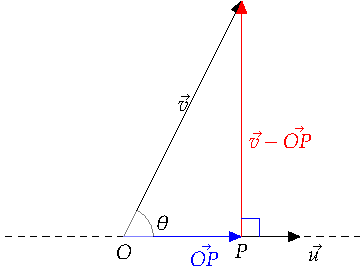
\includegraphics{projecao-vetores-plano-cartesiano.pdf}
  % \begin{tikzpicture}[scale=2]
  %   \coordinate [label=below:$O$] (O) at (0,0);
  %   \coordinate (V) at (1,2);
  %   \coordinate (U) at (1.5,0);
  %   %\coordinate (B) at (0,1);
  %   \coordinate[label=below:$P$] (P) at ($(O)!(V)!(U)$);
  %   %defini\c{c}\~ao das coordenadas dos eixos cartesianos
  %   \coordinate (F) at (-1,0);
  %   \coordinate (X) at (2,0);
  %   % Styles
  %   \tikzstyle{axes}=[]

  %   \begin{scope}[style=axes]%constr\'oi os eixos cartesianos
  %   \draw[dashed] (F) -- (X) coordinate(x axis);
  %   %\draw[->] (G) -- (Y) node[left] {$y$} coordinate(y axis);
  %   \end{scope}

  %   \draw[->,>=triangle 45] (O)--(V)
  %     node[above,midway]{$\vec{v}$};
  %   \draw[->,>=triangle 45] (O)--(U)
  %     node[below right]{$\vec{u}$};
  %   \draw[->,>=triangle 45,blue] (O)--(P)
  %     node[midway,below right]{$\vec{OP}$};
  %   \draw[->,>=triangle 45,red] ($(O)!(V)!(U)$) -- (V)
  %     node[midway,below right]{$\vec{v} - \vec{OP}$};
  %   \draw[anchor=base,color=blue] (P.center)  ++(.15,0)  -- ++(0,0.15) -- ++(-0.15,0);
    
  %   % Mark the angle XAY
  %   \begin{scope}
  %   \path[clip] (O) -- (V) -- (U);
  %   \fill[white, opacity=0.5, draw=black] (O) circle (2.5mm);
  %   \node at ($(O)+(20:3.5mm)$) {$\theta$};
  %   \end{scope}
  % \end{tikzpicture}
\end{figure}

O vetor $\vec{OP}$ \'e paralelo ao vetor $\vec{u}$ e o vetor $\vec{PA}$ \'e ortogonal ao vetor $\vec{u}$.

\begin{definicao}\label{projecao_ortogonal}
  Seja $\vec{u}$ um vetor n\~ao nulo. Dado qualquer vetor $\vec{v}$, o vetor $\vec{OP}$ \'e chamado de \textbf{proje\c{c}\~ao ortogonal} de $\vec{v}$ sobre $\vec{u}$, e \'e indicado por $\proj_{\vec{u}}\vec{v}$ se satisfaz as seguintes condi\c{c}\~oes:\index{Vetores!Proje\c{c}\~ao ortogonal}
  \begin{enumerate}
    \item $\vec{OP} \varparallel\vec{u}$
    \item $(\vec{v} - \vec{OP}) \perp \vec{u}$.
  \end{enumerate}
\end{definicao}

Podemos tamb\'em escrever
\begin{enumerate}
  \item $\proj_{\vec{u}}\vec{v} \varparallel\vec{u}$
    \item $(\vec{v} - \proj_{\vec{u}}\vec{v}) \perp \vec{u}$.
\end{enumerate}

No caso acima temos
\[
  \cos\theta = \dfrac{\norm{\vec{OP}}}{\norm{\vec{v}}}
\]
e ent\~ao $\norm{\vec{OP}} = \norm{\vec{v}}\cos\theta$. Mas
\[
  \cos\theta = \dfrac{\vec{u}\cdot\vec{v}}{\norm{\vec{u}}\norm{\vec{v}}}
\]
e assim podemos escrever
\[
  \norm{\vec{OP}} = \dfrac{\vec{u}\cdot\vec{v}}{\norm{\vec{u}}}.
\]
Al\'em disso, como $\vec{OP}$ \'e paralelo \`a $\vec{u}$ e de mesmo sentido, devemos ter $\vec{OP} = \lambda\vec{u}$ com $\lambda > 0$. Da{\'\i}
$\lambda = \norm{\vec{OP}}/\norm{\vec{u}}$ e ent\~ao
\[
  \vec{OP} = \dfrac{\norm{OP}}{\norm{\vec{u}}^2}\vec{u}.
\]

Esta constru\c{c}\~ao s\'o \'e v\'alida no caso em que o \^angulo $\theta$ entre $\vec{u}$ e $\vec{v}$ satisfaz $0 < \theta < \pi/2$. Nos casos
\begin{figure}
  \centering
  \caption{Vetor proje\c{c}\~ao}
  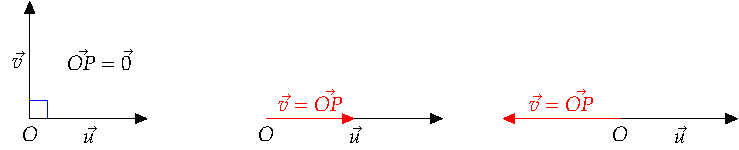
\includegraphics{vetores-projecao-plano-cartesiano.pdf}
  % \begin{tikzpicture}
  %     \coordinate[label=below:$O$] (A) at (-8,0);
  %     \coordinate (X) at (-6,0);
  %     \coordinate (Y) at (-8,2);
  %     \coordinate[label=right:$\vec{OP}\eq \vec{0}$] (P) at (-7.5,1);

  %     \draw[->,>=triangle 45] (A) -- (X)
  %     node[midway,below]{$\vec{u}$};
  %     \draw[->,>=triangle 45] (A) -- (Y)
  %     node[midway,left]{$\vec{v}$};
  %     \draw[anchor=base,color=blue] (A.center)  ++(.3,0)  -- ++(0,0.3) -- ++(-0.3,0);

  %     \coordinate[label=below:$O$] (B) at (-4,0);
  %     \coordinate (C) at (-2.5,0);
  %     \coordinate (D) at (-1,0);

  %     \draw[->,>=triangle 45] (B) -- (D)
  %     node[midway,below]{$\vec{u}$};
  %     \draw[->,>=triangle 45,red] (B) -- (C)
  %     node[midway,above]{$\vec{v} = \vec{OP}$};
      
  %     \coordinate[label=below:$O$] (B) at (2,0);
  %     \coordinate (C) at (0,0);
  %     \coordinate (D) at (4,0);

  %     \draw[->,>=triangle 45] (B) -- (D)
  %     node[midway,below]{$\vec{u}$};
  %     \draw[->,>=triangle 45,color=red] (B) -- (C)
  %     node[midway,above]{$\vec{v} = \vec{OP}$};
  %   \end{tikzpicture}
\end{figure}
n\~ao podemos usar a constru\c{c}\~ao envolvendo o \^angulo $\theta$ entre os vetores.
\begin{proposicao}
  Seja $\vec{u}$ um vetor n\~ao nulo. Qualquer que seja o vetor $\vec{v}$, existe e \'e \'unica a proje\c{c}\~ao ortogonal de $\vec{v}$ sobre $\vec{u}$. Sua express\~ao em termos de $\vec{u}$ e $\vec{v}$ \'e dada por
  \[
    \proj_{\vec{u}}\vec{v} = \dfrac{\vec{u}\cdot\vec{v}}{\norm{\vec{u}}^2}\vec{u}
  \]
  e sua norma \'e dada por
  \[
    \norm{\proj_{\vec{u}}\vec{v}} = \dfrac{\mid\vec{v}\cdot\vec{u}\mid}{\norm{\vec{u}}}.
  \]
\end{proposicao}
\begin{prova}
  Seja $\vec{p} = \proj_{\vec{u}}\vec{v}$. Da Defini\c{c}\~ao \ref{projecao_ortogonal}, dizer que $\vec{p}$ \'e a proje\c{c}\~ao ortogonal de $\vec{v}$ sobre $\vec{u}$ significa que $\vec{p}$ \'e um vetor tal que $\vec{p}\varparallel\vec{u}$ e $(\vec{v} - \vec{p})\perp\vec{u}$.

  Como $\vec{p}\varparallel\vec{u}$, ent\~ao pela Proposi\c{c}\~ao \ref{vetores_paralelos} existe um escalar $\lambda$ tal que $\vec{p} = \lambda\vec{u}$. Assim qualquer vetor do tipo $\lambda\vec{u}$ \'e um candidato para ser a proje\c{c}\~ao ortogonal. Mas, para que $\vec{p}$ seja a proje\c{c}\~ao ortogonal, ele deve satisfazer $(\vec{v} - \vec{p})\perp\vec{u}$. Logo
  \begin{align*}
    (\vec{v} - \vec{p})\perp\vec{u} \Leftrightarrow (\vec{v} - \vec{p})\cdot\vec{u} = 0 \Leftrightarrow \vec{v}\cdot\vec{u} - \lambda\vec{u}\cdot\vec{u} = 0 \Leftrightarrow \lambda = \dfrac{\vec{v}\cdot\vec{u}}{\norm{\vec{u}}^2}.
  \end{align*}
  Assim existe um \'unico $\lambda$ que satisfaz a condi\c{c}\~ao $(\vec{v} - \vec{p})\perp\vec{u}$, e da{\'\i} o vetor $\vec{p}$ \'e \'unico. Portanto
  \[
    \proj_{\vec{u}}\vec{v} = \vec{p} = \dfrac{\vec{v}\cdot\vec{u}}{\norm{\vec{u}}^2}\vec{u}.
  \]
  Al\'em disso
  \[
    \norm{\proj_{\vec{u}}\vec{v}} = \norm{\dfrac{\vec{v}\cdot\vec{u}}{\norm{\vec{u}}^2}\vec{u}} = \dfrac{\mid\vec{v}\cdot\vec{u}}{\norm{\vec{u}}}
  \]
  como quer{\'\i}amos.
\end{prova}

\begin{observacao}
  O escalar $\lambda$ encontrado na proposi\c{c}\~ao anterior pode ser negativo ou zero. Ele ser\'a negativo quando $\pi/2 \le \theta \le \pi$ e ser\'a zero quando $\vec{u}\perp\vec{v}$.
  \begin{figure}[!h]
    \centering
    \caption{Possibilidades para $\lambda$}
    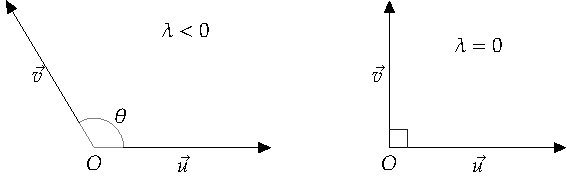
\includegraphics{vetores-projecao-escalar-plano-cartesiano.pdf}
    % \begin{tikzpicture}
    %   \coordinate[label=below:$O$] (A) at (-5,0);
    %   \coordinate (X) at (-2,0);
    %   \coordinate (Y) at (-6.5,2.5);
    %   \coordinate[label=right:$\lambda < 0$] (P) at (-4,2);

    %   \draw[->,>=triangle 45] (A) -- (X)
    %   node[midway,below]{$\vec{u}$};
    %   \draw[->,>=triangle 45] (A) -- (Y)
    %   node[midway,left]{$\vec{v}$};

    %   % Mark the angle XAY
    %   \begin{scope}
    %   \path[clip] (A) -- (X) -- (Y);
    %   \fill[white, opacity=0.5, draw=black] (A) circle (5mm);
    %   \node at ($(A)+(50:7mm)$) {$\theta$};
    %   \end{scope}
      
    %   \coordinate[label=below:$O$] (B) at (0,0);
    %   \coordinate (C) at (3,0);
    %   \coordinate (D) at (0,2.5);
    %   \coordinate[label=below:$\lambda\eq 0$] (Q) at (1.5,2);

    %   \draw[->,>=triangle 45] (B) -- (C)
    %   node[midway,below]{$\vec{u}$};
    %   \draw[->,>=triangle 45] (B) -- (D)
    %   node[midway,left]{$\vec{v}$};
    %   \draw[anchor=base,color=blue] (B.center)  ++(.3,0)  -- ++(0,0.3) -- ++(-0.3,0);

    %   % Mark the angle XAY
    %   % \begin{scope}
    %   % \path[clip] (A) -- (X) -- (Y);
    %   % \fill[white, opacity=0.5, draw=black] (A) circle (5mm);
    %   % \node at ($(A)+(30:7mm)$) {$\theta$};
    %   % \end{scope}
    %   \end{tikzpicture}
  \end{figure}
\end{observacao}

\begin{exemplos}\label{exemplosprojecao}
  \begin{enumerate}
    \item Encontre a proje\c{c}\~ao ortogonal do vetor $\vec{v} = (4, -1)$ sobre o vetor $\vec{u} = (2, 1)$.
    \begin{solucao}
       Temos
       \[
          \proj_{\vec{u}}\vec{v} = \dfrac{\vec{v}\cdot\vec{u}}{\norm{\vec{u}}^2}\vec{u}.
       \]
       Agora
       \begin{align*}
         \vec{u}\cdot\vec{v} = 7\\
         \norm{\vec{u}}^2 = 5
       \end{align*}
       e da{\'\i}
       \[
          \proj_{\vec{u}}\vec{v} = \dfrac{7}{5}(2, 1) = \left(\dfrac{14}{5}, \dfrac{7}{5}\right).
       \]
       Por outro lado,
       \[
          \proj_{\vec{v}}\vec{u} = \dfrac{\vec{u}\cdot\vec{v}}{\norm{\vec{v}}^2}\vec{v}.
       \]
       Agora
       \begin{align*}
         \vec{u}\cdot\vec{v} = \vec{v}\cdot\vec{u} = 7\\
         \norm{\vec{v}}^2 = 17
       \end{align*}
       e da{\'\i}
       \[
          \proj_{\vec{v}}\vec{u} = \dfrac{7}{17}(4, -1) = \left(\dfrac{28}{17}, \dfrac{-7}{17}\right).
       \]
     \end{solucao} 
     \item Considere um tri\^angulo $ABC$ onde $A(3,3)$, $B(0,1)$ e $C(1,6)$.
     \begin{enumerate}\label{exemploprojecao2}
       \item Verifique que $ABC$ \'e um tri\^angulo ret\^angulo em $A$.
       \item Calcule a proje\c{c}\~a do cateto $BA$ sobre a hipotenusa $BC$.
       \item Determine o p\'e da altura do tri\^angulo relativo ao v\'ertice $A$.
     \end{enumerate}
     \begin{solucao}
       Considere o tri\^angulo abaixo
       \begin{figure}[!h]
        \centering
        \caption{Exemplo \ref{exemplosprojecao}, exerc{\'\i}cio \ref{exemploprojecao2}}
        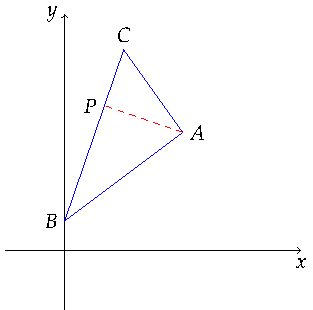
\includegraphics{exemplo-vetores-projecao-plano-cartesiano.pdf}
         % \begin{tikzpicture}[scale=2]
         %    \coordinate (o) at (0,0);
         %    \coordinate[label=right:$A$] (A) at (1,1);
         %    \coordinate[label=left:$B$] (B) at (0,0.25);
         %    \coordinate[label=above:$C$] (C) at (0.5,1.7);
         %    \coordinate[label=left:$P$] (P) at ($(C)!(A)!(B)$);
         %    %defini\c{c}\~ao das coordenadas dos eixos cartesianos
         %    \coordinate (F) at (-0.5,0);
         %    \coordinate (G) at (0,-0.5);
         %    \coordinate (X) at (2,0);
         %    \coordinate (Y) at (0,2);
         %    % Styles
         %    \tikzstyle{axes}=[]

         %    \begin{scope}[style=axes]%constr\'oi os eixos cartesianos
         %    \draw[->] (F) -- (X) node[below] {$x$} coordinate(x axis);
         %    \draw[->] (G) -- (Y) node[left] {$y$} coordinate(y axis);
         %    \end{scope}

         %    \draw[blue] (B)--(A);
         %    \draw[blue] (B)--(C);
         %    \draw[blue] (A)--(C);
         %    \draw[red,dashed] (A) -- ($(C)!(A)!(B)$);
         %  \end{tikzpicture}
       \end{figure}
       \begin{enumerate}
         \item Basta verificar que $\vec{AB}\perp\vec{AC}$. Assim como $\vec{AB} = (-3,-2)$ e $\vec{AC} = (-2,3)$ temos
         \[
            \vec{AB}\cdot\vec{AC} = (-3)(-2) + (-2)3 = 0.
         \]
         Logo $ABC$ \'e um tri\^angulo ret\^angulo.
         \item Temos $\vec{BA} = (3,2)$ e $\vec{BC} = (1,5)$. Da{\'\i}
         \[
            \proj_{\vec{BC}}\vec{BA} = \dfrac{\vec{BC}\cdot\vec{BA}}{\norm{\vec{BC}}^2}\vec{BC} = \dfrac{(3,2)\cdot(1,5)}{\norm{(1,5)}^2}(1,5) = \dfrac{13}{26}(1,5).
         \]
         Assim $\proj_{\vec{BC}}\vec{BA} = \left(\dfrac{1}{2},\dfrac{5}{2}\right)$.
         \item Seja $P(x_1, y_1)$ o p\'e da altura do tri\^angulo $ABC$ relativo ao v\'ertice $A$. Ent\~ao
         \begin{align*}
           \vec{BP} = \proj_{\vec{BC}}\vec{BA}\\
           (x_1, y_1 - 1) = \left(\dfrac{1}{2}, \dfrac{5}{2}\right).
         \end{align*}
         Logo $P\left(\dfrac{1}{2},\dfrac{7}{2}\right)$.
       \end{enumerate}
     \end{solucao}
  \end{enumerate}
\end{exemplos}
% subsection projecao_de_vetores (end)
% chapter vetores (end)